% Magic Comments
% !TeX spellcheck = en_GB
% !TeX encoding = utf8
% !TeX program = pdflatex

\documentclass[12pt, oneside]{amsart}

\usepackage{amssymb}
\usepackage[
    style=numeric-comp,
    backend=biber,
    sorting=nty,
    doi=false,
    isbn=false, 
    natbib=true]{biblatex}
\addbibresource{references.bib}
\emergencystretch=1em

\usepackage{mathtools}
\usepackage{xcolor}
\usepackage{url} % Makes urls nicer
\usepackage[breaklinks=true]{hyperref}
\usepackage{cleveref}

% For tabular
\usepackage{booktabs}
\usepackage{array}
\usepackage{adjustbox}
\usepackage{multirow}
\usepackage{makecell}

% For figures
\usepackage{graphicx}

% Floating for positioning environments
\usepackage{float}


\newtheorem{thm}{Theorem}[section]
\newtheorem{prop}[thm]{Proposition}
\newtheorem{lem}[thm]{Lemma}
\newtheorem{cor}[thm]{Corollary}

\theoremstyle{definition}
\newtheorem{definition}[thm]{Definition}

\theoremstyle{remark}
\newtheorem{remark}[thm]{Remark}

\numberwithin{equation}{section}


% Package specific things

% TODO: Do we want to have equations just labeled with "(3.1)" or with 
% TODO: "equation 3.1".
%\crefname{equation}{equation}{equations} 
%\Crefname{equation}{Equation}{Equations}
\crefname{equation}{}{} 
\Crefname{equation}{}{}

\crefname{table}{table}{tables}
\Crefname{table}{Table}{Tables}

\crefname{figure}{figure}{figures}
\Crefname{figure}{Figure}{Figures}


% Definitions
\newcommand{\defn}{\ensuremath{:=}}
\newcommand{\revdefn}{=:}

% Sets
\newcommand{\R}{\mathbb{R}}
\newcommand{\N}{\mathbb{N}}
\newcommand{\Z}{\mathbb{Z}}
\newcommand{\C}{\mathbb{C}}
\newcommand{\Q}{\mathbb{Q}}
\newcommand{\T}{\mathbb{T}}

% Caligraphic
\newcommand{\cO}{\mathcal{O}}
\newcommand{\cZ}{\mathcal{Z}}
\newcommand{\cP}{\mathcal{P}}
\newcommand{\cI}{\mathcal{I}}
\newcommand{\cA}{\mathcal{A}}

% Function Spaces
\newcommand*{\pols}[2][]{\ensuremath{\cP^{#1}\left(#2\right)}}

% bold
\newcommand{\ZZ}{\ensuremath{\mathbf{Z}}}
\newcommand{\FF}{\ensuremath{\mathbf{F}}}
\newcommand{\XX}{\ensuremath{\mathbf{X}}}

% Set brackets
\newcommand{\set}[1]{\left\{#1\right\}}

% Make index set from 1 to (inclusive) m:
\newcommand*{\indexset}[2][1]{[#1:#2]}

% Make a colon: (Used for defining a function from A to B)
\newcommand*{\from}{\colon}

% Probability commands: Expectation, Variance, Covariance, Bias
\newcommand{\E}{\mathbb{E}}

% Vector Norm
\newcommand{\norm}[2][2]{\left\lVert#2\right\rVert_{#1}}

% Derivatives
\newcommand{\deriv}[2][x]{\frac{\mathrm{d}}{\mathrm{d}#1} (#2)}

% Partial derivatives
\newcommand{\pderiv}[2]{\frac{\partial #1}{\partial #2}}

% Integral 
\newcommand{\integral}[4]{\int\limits_{#1}^{#2}#3~\mathrm{d}#4}

% Inner product
\newcommand{\inner}[2]{\left\langle#1,#2\right\rangle}

% Absolute value
\newcommand{\abs}[1]{\left \vert #1 \right \vert }

% If else (ternary operator)
\newcommand{\ifelse}[3]{#1~\textrm{if}~#2~\textrm{else}~#3}

% Vector-Arrow
\newcommand{\vecarrow}[1]{\vec{#1}}

% Vector 2 dimensions
\newcommand{\vtwo}[2]{\left(\begin{array}{c}#1\\#2\end{array}\right)}

% Vector 3 dimensions
\newcommand{\vthree}[3]{\left(\begin{array}{c}#1\\#2\\#3\end{array}\right)}

% Large Limit bar for defined integral borders
\newcommand{\eval}[2]{\Biggr|_{#1}^{#2}}

% Divides symbol
\newcommand{\divides}{\vert}

% Changing greek letters
\let\uglyepsilon\epsilon % Still saving the previous one
\let\epsilon\varepsilon

\let\otherphi\phi % Still saving the previous one
\let\phi\varphi

% Images from inkscape

\newcommand{\incfig}[2][\columnwidth]{%
	\def\svgwidth{#1}
	\import{../figures/}{#2.pdf_tex}
}

\renewcommand*{\aa}{\mathbf{a}}

\renewcommand*{\Re}{\mathrm{Re}}
\renewcommand*{\Im}{\mathrm{Im}}

%Shortcuts
\renewcommand{\d}{\mathrm{d}}

% Mathematical Operators:
\DeclareMathOperator*{\supp}{supp} % support of a vector
\DeclareMathOperator*{\argmin}{argmin}
\DeclareMathOperator*{\spn}{span}
\DeclareMathOperator{\id}{id}
\DeclarePairedDelimiter\ceil{\lceil}{\rceil}
\DeclarePairedDelimiter\floor{\lfloor}{\rfloor}

% For tabulars
\newcommand{\first}[1]{\textbf{#1}}

% Quotation marks
\newcommand*{\quotes}[1]{``#1''}


% Comments
\newcommand*{\jakob}[1]{\color{red} \textbf{\emph{#1}} \color{black}}
\newcommand*{\elias}[1]{\color{blue} \textbf{\emph{#1}} \color{black}}
\newcommand*{\mario}[1]{\color{green} \textbf{\emph{#1}} \color{black}}

% %%%%%%%%%%%%%%%%%%%%%%%%%%%%%%%%%%%%%%%%%%%%%%%%%%%%%%%%%%%%%%%%% %

\begin{document}
\title{Least Squares and Smolyak's Algorithm}


\author{Jakob Eggl, Elias Mindlberger and Mario Ullrich}
\date{\today}
\keywords{Polynomial interpolation, Sparse-Grids, Least-Squares, Smolyak} % 

%\author{Jakob Eggl}
%\address{Institute of Analysis, Johannes Kepler University Linz, Austria.}
%\email{jakob.eggl@jku.at}
%
%\author{Elias Mindlberger}
%\address{Institute of Analysis, Johannes Kepler University Linz, Austria.}
%\email{elias.mindlberger@jku.at}
%
%\author{Mario Ullrich}
%\address{Institute of Analysis, Johannes Kepler University Linz, Austria.}
%\email{mario.ullrich@jku.at}

% \thanks{\(\star\) Equal Contribution.}


\begin{abstract}
We present novel, large-scale experiments for polynomial interpolation in high 
dimensional settings using some of the most popular algorithms available. We 
compare Smolyak's Algorithm (SA) on sparse grids and Least Squares (LSQ) using 
random data. We empirically confirm that interpolation using LSQ performs 
equally as good on smooth and better on non-smooth functions if SA is given 
\(n\) and LSQ is given \(2 \cdot n\) points.
\end{abstract}

\maketitle

%\tableofcontents

%%%%%%%%%%%%%%%%%%%%%%%%%%%%%%%%%%%%%%%%%%%%%%%%%%%%%%%%%%%
\section{Introduction}
%%%%%%%%%%%%%%%%%%%%%%%%%%%%%%%%%%%%%%%%%%%%%%%%%%%%%%%%%%%

Smolyak's algorithm on Sparse Grids has been of high theoretical and practical 
interest for a long time \cite{BarthelmannHighDim_2000,smolyak1963,Coleman_SmoylakGithub_2013,JuddSmolyak_2014}. In \cite{Krieg_2020}, it was recently found that Smolyak's algorithm is \emph{not} optimal in the sampling numbers
\[
    e_n(H) \defn \inf_{\substack{x_1, \dots, x_n \in D \\ \phi_1, \dots, \phi_n 
    \in L_2}} \sup_{f \in B(H)} \norm[L_2]{f - \sum_{i=1}^n f(x_i) \phi_i}
\]
disproving conjecture 5.26 in \cite{Dung_Temlyakov_Ullrich_2018}. We extend upon these theoretical findings with an empirical study comparing the performance of Smolyak's algorithm and Least Squares on simple function recovery problems on the unit cube. Our implementation is available at \url{https://github.com/th3lias/NumericalExperiments}.


%%%%%%%%%%%%%%%%%%%%%%%%%%%%%%%%%%%%%%%%%%%%%%%%%%%%%%%%%%%
\section{Notation}
%%%%%%%%%%%%%%%%%%%%%%%%%%%%%%%%%%%%%%%%%%%%%%%%%%%%%%%%%%%

We denote the indexset containing all indices $i\in \Z$ 
where $m\leq i\leq n$ for $m\leq n$ with \(\indexset[m]{n}\). For the set of 
polynomials \(p\) from \(D \subseteq \C^K,\, K \in \N\) to the field \(\F\) of maximal 
degree \(N\) we use the notation 
\(p \in \pols[N]{V, \F}\).
We use \(f \lesssim g\) to denote \(f \leq c 
g\) for functions \(f, g\). With \(B(X)\) we denote the closed unit ball of a 
normed space \(X\). With \(X^\star\) we denote the topological dual space of \(X\).
\newpage
%%%%%%%%%%%%%%%%%%%%%%%%%%%%%%%%%%%%%%%%%%%%%%%%%%%%%%%%%%%
\section{Interpolation}
%%%%%%%%%%%%%%%%%%%%%%%%%%%%%%%%%%%%%%%%%%%%%%%%%%%%%%%%%%%

Given \(i \in \N\) and distinct data points \(\XX_i \defn \set{x_{i, 0}, \dots, 
x_{i, n}} \subseteq D \subseteq \R\) \jakob{$D_i$ here?}, function values 
\(\YY_i \defn \set{y_{i, 0}, \dots, y_{i, n}} = \set{f(x_{i, 0}), \dots, 
f(x_{i, n})} \subseteq \R\) for \(f: D_i \to \R\), it is a well known fact that 
there exists a polynomial \(\cI(\ZZ_i)\) of degree \(n\) such that \[
    \cI(\ZZ_i) = y_{i, j},\quad j \in \indexset[0]{n}.
\]
for \(\ZZ_i \defn (\XX_i, \YY_i)\)
We then call \(\cI(\ZZ_i)\) an \emph{interpolating} polynomial. It can be written down explicitly as \begin{equation}\label{interpolating_polynomial}
    \cI(\ZZ_i) = \sum_{j=0}^n y_{i, j} \ell_{i, j}
\end{equation}
for basis functions \(\ell_{i, j} \in \pols[n]{\R, \R}\). Moreover, in a single 
dimension, the formula for this basis is
\[
\ell_{i, j}(w) = \prod_{m \in \indexset[0]{n} \setminus \set{j}} \frac{w-x_{i, 
m}}{x_{i, j}-x_{i, m}},
\]
see \cite{waring1779, lagrange1901}. We call \(\cI\) the 
\emph{Lagrange interpolator}.

Suppose now we have \(d\) point sets \(\XX_i\). By taking the full cartesian product of point sets \[
    \XX \defn \bigtimes_{i=1}^d \XX_i,
\] we may identify our grid by \(\XX = \set{\bfx_\bfj}_{\bfj}\) with \(\bfj \in \set{0,1,\dots,n}^d\) and suppose we have according function evaluations \(\YY \defn \set{y_\bfj}_\bfj = \set{f(\bfx_\bfj)}_\bfj\) for \(f: D \to \R\), \(D \subseteq \R^d\). Let \(\ZZ \defn (\XX, \YY)\). Then, we may construct an interpolating polynomial as in \cref{interpolating_polynomial}. Indeed, the general formula stays the same but we take tensor product of basis functions, i.e. \begin{equation}\label{multivariateLagrange}
    \ell_\bfj(\bfw) = \bigotimes_{i=1}^d \ell_{j_i}(w_i) = \prod_{i=1}^d \ell_{j_i}(w_i) = \prod_{i=1}^d \prod_{\substack{k=0 \\ k \neq j_i}}^n \frac{w_i - x_{i, k}}{x_{i, j_i} - x_{i, k}}
\end{equation}
and the sum now ranges over all multiindices \(\bfj = (j_1, \dots, j_d) \in \N_0^d\) with \(\bfj \in \set{0, 1, \dots, n}^d\). We denote \begin{equation}\label{eq:interpolantdD}
	\cI(\ZZ) \defn \sum_{j_1 = 0}^n \cdots \sum_{j_d = 0}^n y_{j_1, \dots, j_d} \ell_{j_1, \dots, j_d}
\end{equation}
for the interpolant on \(\R^d\).
Formula \ref{multivariateLagrange} is not a great choice for performing calculations on hardware. Leaving the storage of \((n+1)^d\) grid points aside, for computing one evaluation of the map \(\bfw \mapsto \cI(\ZZ)(\bfw)\), one must compute the sum of \((n+1)^d\) terms, where in each summand, the evaluation of \(d\) basis functions is computed, each of which is a product of \(n\) terms. This evaluation is thus as costly as \(\cO((n+1)^d d n)\). One can counter the costly computation of the interpolating polynomial at a given point by reformulating the above (numerically instable) Lagrange interpolator in it's barycentric form
\begin{equation}\label{eq:multivarBarycentric}
    \cI(\ZZ)(\bfw) = \frac{\sum_{j_1=0}^{n} \ell^{(1)}_{j_1}(w_1) \cdots \sum_{j_d=0}^{n} \ell^{(d)}_{j_d}(w_d) y_\bfj}{\sum_{j_1=0}^{n} \ell^{(1)}_{j_1}(w_1) \cdots \sum_{j_d=0}^{n} \ell^{(d)}_{j_d}(w_d)}
\end{equation}
where
\begin{equation}\label{eq:barycentricBasis}
    \ell^{(k)}_{j_k}(w) \defn \frac{m_{j_k}}{w-x_{j_k}} \mid k \in \indexset[1]{d}.
\end{equation}
with \(x_{j_k}\) being the \(j_k\)--th entry of \(\bfx\). \(m_{j_k}\) are the \emph{barycentric} weights which can be computed in \(\cO(n^2)\) time for general point distributions but admit \(\cO(1)\) computation for well--known and widely used point sets \cite{klimke2004}. For example, due to \cite{Berut_2004},
\begin{equation}\label{barycentric_weights_chebyshev}
    m_{0} = \frac{1}{2},\quad m_{l} = (-1)^l,\, l \in \indexset[1]{n-1},\quad m_n = \frac{1}{2}(-1)^n
\end{equation}
for the \emph{Chebyshev Gauss-Lobatto} (or just Chebyshev extrema), in which \begin{equation}\label{ChebyshevGaussLobatto}
    x_l \defn x_{l,n} \defn - \cos\frac{l \pi}{n},\, l \in \indexset[0]{n}.
\end{equation}

Similarly, for the \emph{Chebyshev points of the second kind}
\begin{equation}\label{eq:chebyPts2}
    x_l = x_{l, n} = \cos \frac{l \pi}{n},\, l \in \indexset[0]{n}
\end{equation}
one gets the closed form
\begin{equation}\label{eq:weightsChebyshev}
    m_l = {\left(-1\right)}^l \cdot \begin{cases}
        1/2 &l \in \set{0, n}\\
        1 &\text{else.}
    \end{cases}
\end{equation}
In this case, one achieves an evaluation time of \(\cO((n+1)^d)\).
Hence, in this construction, one cannot get around this bottleneck. 
\jakob{Here, equation \cref{eq:chebyPts2} and \cref{eq:weightsChebyshev} are 
the same point set. This is probably wrong.}


%%%%%%%%%%%%%%%%%%%%%%%%%%%%%%%%%%%%%%%%%%%%%%%%%%%%%%%%%%%
\section{Smolyak's Algorithm \& Sparse Grids}
%%%%%%%%%%%%%%%%%%%%%%%%%%%%%%%%%%%%%%%%%%%%%%%%%%%%%%%%%%%

The following description follows \cite{BarthelmannHighDim_2000}.
The question arises, how one may reduce the complexity of exact interpolation 
on grids. The central idea of sparse grids is to \emph{not} take the full 
tensor product of one dimensional point sets but restrict the number of 
simultaneously \jakob{equally?} large directions. To that end, take a variable 
number of points in each direction, i.e.\ let \(\XX_j \defn \set{x_{1, j}, 
\dots, x_{N(j), j}}\) and \(\cI_j\) the corresponding one--dimensional 
interpolator with \(\cI_0 \defn 0\), \(\Delta_j \defn \cI_j - \cI_{j-1}\). Then 
Smolyak's algorithm is given in a simple recursive manner
\begin{equation}\label{Smolyak}
    \cA(q, d) \defn \sum_{\norm[1]{\bfj} \leq q} \bigotimes_{k=1}^d \Delta_{j_k} = \cA(q-1, d)+\sum_{\norm[1]{\bfj}=q} \bigotimes_{k=1}^d \Delta_{j_k}
\end{equation}
with \(\cA(q, d) = 0,\, q < d\) and \(\bfj\), \(\cI\) as before. Evidently, only a relatively small number of knots, through the restriction \(\norm[1]{\bfj} \leq q\), is needed. To be precise, \(\cO(n (\log n)^{d-1})\) points are needed. Hence \(q\) can be thought of as a resolution parameter. By this form, one only needs to assess the function values at the \emph{sparse grid} \[
	H(q, d) \defn \bigcup_{q-d+1 \leq \norm[1]{\bfj} \leq q} \XX_{j_1} \times \cdots \times \XX_{j_d}
\]
where the number of nodes in a given direction can never be \emph{large} for all directions simultaneously. Hence, given that \(\XX_j \subset \XX_{j+1}\), one may write the interpolator given by Smolyak's construction as \[
	\cA(q, d)(f) = \sum_{\norm[1]{\bfj} \leq q} f(\bfx_\bfj) \ell_\bfj,
\]
which is familiar from before.
The number of knots \(N(j)\) used for each one--dimensional interpolation rule \(\cI_j\) remains to be specified. In order to obtain nested points, i.e. \(\XX_j \subset \XX_{j+1}\) and thus \(H(q, d) \subset H(q+1,d)\) together with collocation rules such as \cref{ChebyshevGaussLobatto} or \cref{eq:chebyPts2} it is usual to choose a doubling rule, i.e. \[
	N(1) = 1,\quad N(j) = 2^{j-1}+1,\, j > 1.
\]

\subsection{Polynomial Exactness}
Without loss of generality, we restrict ourselves to the symmetric cube \([-1, 
1]^d\) \jakob{We have $[0,1]^d$. It appears multiple times, therefore I didn't 
want to erase it everywhere now.} for interpolation of unknowns instead of a 
general domain \(D\). In this 
case, Smolyak's algorithm is well known to exactly reproduce functions on 
certain polynomial spaces given that the rules \(\cI_j\) are exact on nested 
spaces \(V_j\), see \cite{DELVOS198299} or \cite{novakRitter1996}.
\begin{lem}
	Assume \(\cI_j\) is exact on the vector space \(V_j \subseteq C([-1, 1])\) and assume \[
		V_1 \subset V_2 \subset V_3 \subset \dots,
	\]
	then \(\cA(q, d)\) is exact on \[
		\sum_{\norm[1]{j}=q} V_{j_1} \otimes \cdots \otimes V_{j_d}
	\]
\end{lem}
\cite{BarthelmannHighDim_2000} showed the following. \jakob{Maybe cite 
\cite{BarthelmannHighDim_2000} directly in the lemma environment. I.e. 
begin{lem}[cf. \cite{BarthelmannHighDim_2000}]}
\begin{lem}
	\(\cA(q, d)\) is exact on \[
		E(q, d) \defn \sum_{\norm[1]{\bfj} = q} \pols[m_{j_1}-1]{\R, \R} \otimes \cdots \otimes \pols[m_{j_d}-1]{\R, \R}
	\]
	and \(\cA(d+k, d)\) is exact for all polynomials of degree \(k\).
\end{lem}
Indeed, the following also follows from \cite{BarthelmannHighDim_2000}. Note that we now abuse the notation from \ref{interpolating_polynomial} by writing \(\cI(\ZZ) \revdefn \cI(f, \XX) \revdefn \cI(f)\).
\begin{lem}
	Assume \(\XX_1 \subset \XX_2 \subset \dots\) and \(\cI_j(f)(x) = f(x)\) for every \(f \in C([-1, 1])\) and every \(x \in \XX_j\). Then \[
		\cA(q, d)(f)(x) = f(x)
	\]
	for every \(f \in C([-1, 1]^d)\) and \(x \in H(q, d)\).
\end{lem}

\subsection{Error Bounds}
Since the interpolation operator \(\cI_j\) as defined before is exact on \(\pols[N(j)-1]{\R, \R}\) one concludes \[
	\norm[\infty]{f - \cI_j(f)} \leq \err_{N(j)-1}(f)(1+\Lambda_{N(j)})
\]
where \(\err_n\) is the error of the best approximation by \(p \in \pols[n]{\R, \R}\), \(\Lambda_n\) is the Lebesgue constant for the point set in \Cref{ChebyshevGaussLobatto} and \(n \geq 2\), in which case it is known that \[
	\Lambda_n \leq \frac{2}{\pi} \log(n-1)+1,
\]
see for example \cite{zeller1966} and \cite{Dzjadyk1983}. The following bounds can be found in \cite{BarthelmannHighDim_2000} and is well known since \cite{smolyak1963, temlyakov1986, WASILKOWSKI19951}.

\begin{lem}
	For the space
	\[
		F_d^k \defn \set{f: [-1, 1]^d \to \R \mid D^\alpha f \text{ continuous if } \alpha_i \leq k \text{ for all } i}
	\]
	the error of \(\cA(q, d)\) can be bounded as \[
		\norm[\op]{I_d - \cA(q, d)} \leq c_{d,k} n^{-k} \left(\log n\right)^{(k+2)(d-1)+1}
	\]
	where \(I_d\) is the embedding \(F_d^k \hookrightarrow C([-1, 1]^d)\) and \(c_{d, k}\) is a positive constant only dependent on \(d\) and \(k\).
\end{lem}

Moreover, for the Sobolev--Hilbert space \(H_w^k\) with \begin{equation}
	H_w^k \defn \set{f \in L^2_w : \norm[k]{f}^2 = \sum_{\ell \in \N_0} (1+\ell^2)^k \inner{f}{b_\ell}^2 < \infty}
\end{equation}
with \(\inner{f}{b_\ell}\) being the \(\ell\)--th Fourier coefficient, one obtains \[
	\norm[0]{f-\cA(q, d)(f)} \leq c_{d, k} n^{-k} \left(\log n\right)^{(k+1)(d-1)}\norm[k]{f}.
\]
Here, \(L^2_w\) is the \(L^2\) weighted by the Chebyshev weight \begin{equation}\label{chebyshev_weight}
	\left(1-x^2\right)^{-1/2}.
\end{equation}
In that case, it is well known that the Chebyshev polynomials
\begin{equation}\label{chebyshev_polynomials}
	T_n(x) \defn \cos(n \arccos(x)).
\end{equation}
form an orthonormal basis.

%%%%%%%%%%%%%%%%%%%%%%%%%%%%%%%%%%%%%%%%%%%%%%%%%%%%%%%%%%%
\section{Least Squares}
%%%%%%%%%%%%%%%%%%%%%%%%%%%%%%%%%%%%%%%%%%%%%%%%%%%%%%%%%%%

Contrary to the construction of exactly interpolating approximants in the case 
of Smolyak's algorithm, Least Squares is a conceptually simpler algorithm. We 
are given the overdetermined system \[
    A\bfz = \bfy
\]
where \(A \in \R^{n \times m}\) with \(n > m\). It is well--known that this system may be inconsistent and no exact solution exists. However, one may always pose the optimisation problem solving for \(\bfz \in \R^{m}\) with the smallest error
\begin{equation}\label{eq:leastSquares}
    \inf_{\bfz \in \R^{m}} \norm[]{A\bfz - \bfy}.
\end{equation}
It is further known that, in case of a full--rank matrix \(V\), the unique 
solution to \Cref{eq:leastSquares} is given by 
\begin{equation}\label{eq:ls_solution_moore_penrose_inverse}
	\bfz_* = \left(A^\top A\right)^{-1} A^\top \bfy \in \R^m.
\end{equation}
In our specific case of polynomial interpolation, \(A\) is the Vandermonde 
matrix, consisting of basis polynomials \(b_1, b_2, \dots, b_m\) evaluated at 
the $n$ different sampled points \(x_1, x_2, \dots, x_n\) in \(D \subseteq 
\R^d\) and \(\bfy\) is the vector of function values sampled from the unknown 
function \(f\from D \to \R\), i.e.\ \(\bfy = \left(f(\bfx_j)\right)_{j=1}^n\). 
As for such points, the Vandermonde matrix is never singular, the solution to 
the approximation problem \[
    \inf_{p} \norm[]{f-p}
\]
can analytically be expressed as \[
    p_* \from D \to \R,\quad t \mapsto \sum_{j=1}^m z_{*_{j}} b_j(t)
\]
where \(\bfz_* = \left(z_{*_j}\right)_{j=1}^m\) is given by 
\Cref{eq:ls_solution_moore_penrose_inverse}.
For the later implementation, we choose the basis polynomials \(b_j\) as the \(j\)--th weighted Chebyshev polynomial \Cref{chebyshev_polynomials}.

%%%%%%%%%%%%%%%%%%%%%%%%%%%%%%%%%%%%%%%%%%%%%%%%%%%%%%%%%%%
\section{Theoretical Guarantees}
%%%%%%%%%%%%%%%%%%%%%%%%%%%%%%%%%%%%%%%%%%%%%%%%%%%%%%%%%%%

% TODO: Eventuell diesen Abschnitt an ein Banachraum Setting anpassen, wie in https://arxiv.org/pdf/2401.02220.

The notation in the following is borrowed from \cite{Ullrich_2020}.
In this section we introduce a formal setting to the former considerations. That is, we consider a Hilbert space \(H\) of real-valued functions on a set \(D\) such that point evaluation \(\delta_x: f \mapsto \int_D f\ \d \delta_x = f(x)\)
is a bounded, linear functional on \(H\).
The general formulation of Least Squares allows for a broad class of recovery 
problems. In our specific case, the function recovery of real--valued functions 
on a \(d\)--dimensional (compact) subset \(D\) using basis functions of a 
\(k\)--dimensional subspace \(V_k \defn \spn \set{b_1, \dots, b_k}\), we 
consider the specific form of Least Squares, given by\[
    A_{n, k}(f) \defn \argmin_{g \in V_k} \sum_{i=1}^n \frac{\abs{g(x_i) - f(x_i)}^2}{\varrho_k(x_i)}
\]
where \[
    \varrho_k(x) = \frac{1}{2} \left( \frac{1}{k} \sum_{j < k} b_{j+1}(x)^2 + \frac{1}{\sum_{j \geq k} a_j^2} \sum_{j \geq k} a_j^2 b_{j+1}(x)^2 \right)
\]
and \(x_1, \dots, x_n \in D\). Whenever \(f \in V_k\), then, of course, \(f = A_{n, k}(f)\). With
\begin{equation}\label{eq:worstCaseError}
    e\left(A_{n,k}, H\right) \defn \sup_{f \in B(H)} \norm[L_2]{f - A_{n,k}(f)},
\end{equation}
we denote the worst case error of \(A_{n,k}\), where we measure the error of the reconstruction in the space \(L_2 \defn L_2(D, \Sigma, \mu)\) of square integrable functions on \(D\) with respect to the measure \(\mu\), such that \(H\) is embedded into \(L_2\). In light of this, the \(n\)--th minimal error (also called \(n\)--th sampling number) is denoted by \[
    e_n(H) \defn \inf_{\substack{x_1, \dots, x_n \in D \\ \phi_1, \dots, \phi_n 
    \in L_2}} \sup_{f \in B(H)} \norm[L_2]{f - \sum_{i=1}^n f(x_i) \phi_i}
\]
and can be understood as the worst case error of the optimal algorithm using \(n\) function values. We get the clear inequality \(e_n(H) \leq e(A_{n,k}, H)\) for any point set \(\set{x_1, \dots, x_n}\). With \[
    a_n(H) \defn \inf_{\substack{h_1^\star, \dots, h_n^\star \in H^\star \\ 
    \phi_1, \dots, \phi_n \in L_2}} \sup_{f \in B(H)} \norm[L_2]{f - 
    \sum_{i=1}^n h_i^\star(f) \phi_i}
\]
we denote the \(n\)-th approximation number, which is the worst-case error of 
an optimal algorithm that uses the \(n\) best arbitrary linear and bounded 
functionals as information about the unknown. This quantity is equal to the 
\(n\)-th singular value of the embedding \(\id\from H \to L_2\).

The following is known since \cite{Krieg_2020}.
\begin{thm}[Krieg--Ullrich]\label{thm:kriegUllrich2020}
    There exist constants \(C, c > 0\) and a sequence of natural numbers \((k_n)\) with each \(k_n \geq cn/\log(n+1)\) and for any \(n \in \N\) and measure space \((D, \Sigma, \mu)\), and any RKHS \(H\) of real-valued functions on \(D\) embedded into \(L_2(D, \Sigma, \mu)\), we have \[
        e_n(H) \leq \sqrt{\frac{C}{k_n} \sum_{j \geq k_n} a_j(H)^2}.
    \]
\end{thm}
In particular, for 
\begin{equation}\label{eq:orderOfApproximationNumbers}
    a_n(H) \lesssim n^{-s} \log^{\alpha + s}(n)
\end{equation}
with \(s > 1/2, \alpha \in \R\), this implies \[
    e_n(H) \lesssim n^{-s} \log^{\alpha+s}(n).
\]
The following follows from \cite{Ullrich_2020}.
\begin{thm}[Ullrich]
    Given \(n \geq 2\) and \(c > 0\), let \[
        k_n \defn \floor*{\frac{n}{2^8 (2+c) \log n}},
    \]
    then, for any measure space \((D, \Sigma, \mu)\) and any RKHS \(H\) of real-valued functions on \(D\), embedded into \(L_2(D, \Sigma, \mu)\), it holds that \[
        e_n\left(A_{n, 2 k_n}, H\right) \leq \sqrt{ \frac{2}{k_n} \sum_{j > k_n} a_j(H)^2 }
    \]
    with probability at least \(1-8n^{-c}\).
\end{thm}

\subsection*{Examples}
In particular, \Cref{eq:orderOfApproximationNumbers} is satisfied for the 
approximation numbers on the Sobolev space of dominating mixed smoothness, 
\begin{align*}
    H &\defn H_{\text{mix}}^s\left(\T^d\right)\\
    &\defn \set{f \in L_2\left(\T^d\right) : \norm[H]{f}^2 \defn \sum_{m \in 
    \N_0^d} \prod_{j=1}^d (1+\abs{m_j}^{2s}) \inner{f}{b_m}^2_{L_2} < \infty}
\end{align*}
with \(\T^d \cong [0, 1)^d\) 
where \(b_m \defn \otimes_{j=1}^d b_{m_j}^{(1)}\) and \(m = (m_1, \dots, m_d)\) with \begin{align*}
    b_{2m}^{(1)} &\defn \sqrt{2}\cos(2\pi m x)\\
    b_{2m-1}^{(1)} &\defn \sqrt{2}\sin(2\pi m x)
\end{align*}
and \(b_0^{(1)} \defn 1\). This satisfies the assumption for \(s > 1/2\). In 
particular, we can say
\begin{equation}\label{eq:conclusio}
    e_n\left( H_{\text{mix}}^s\left(\T^d\right) \right) \lesssim n^{-s}\log^{sd}(n)
\end{equation}
whenever \(s > 1/2\). This disproves a previously posted conjecture (Conjecture 
5.26) in \cite{Dung_Temlyakov_Ullrich_2018} and shows that Smolyak's algorithm 
is not optimal in this case. The surprising fact is that, despite an optimal, 
deterministic construction of the point sets used for reconstruction being 
unknown, random i.i.d. points suffice for a reconstruction error that is on the 
order of optimal points, with probability tending to \(1\). We verify this by 
our experimental findings, presented in \Cref{sec:experimentalFindings} with a 
much better relative number of points used for LSQ function recovery vs. SA 
recovery than guaranteed in this section, i.e. better constants than explicitly 
known before. It remains an open problem to rigorously improve upon the 
constants in \Cref{eq:conclusio}.
%%%%%%%%%%%%%%%%%%%%%%%%%%%%%%%%%%%%%%%%%%%%%%%%%%%%%%%%%%%
\section{Experimental Findings}\label{sec:experimentalFindings}
%%%%%%%%%%%%%%%%%%%%%%%%%%%%%%%%%%%%%%%%%%%%%%%%%%%%%%%%%%%

% TODO: Add what computer and software we used etc. Also how much RAM was used
% TODO: And also, how long it took.

For assessing the performance of the Least Squares algorithms in comparison to 
the Sparse Grid alternative, we use the following $12$ families of test 
functions from \cite{Simulationlib_2013}, each defined of the $d$-dimensional 
unit-cube $[0,1]^d$.

{
	\allowdisplaybreaks[4]
	\begin{align*}
		\begin{array}{l l}
			\text{1. Continuous:} & f_1(x) = \exp\left( - 
			\sum_{i=1}^{d} c_i \abs{x_i - w_i} \right) \\[12pt]
			\text{2. Corner Peak:} & f_2(x) = \left( 1 + 
			\sum_{i=1}^{d} c_i x_i 
			\right)^{-(d+1)} \\[12pt]
			\text{3. Discontinuous:} & f_3(x) = 
			\begin{cases}
				0, &x_1 > w_1 \lor x_2 > w_2, \\
				\exp\left( \sum_{i=1}^{d} c_i x_i \right), & 
				\text{else}
			\end{cases} \\[12pt]
			\text{4. Gaussian:} & f_4(x) = \exp\left( - 
			\sum_{i=1}^{d} c_i^2 (x_i 
			- w_i)^2 \right) \\[12pt]
			\text{5. Oscillatory:} & f_5(x) = \cos\left( 2\pi w_1 + 
			\sum_{i=1}^{d} c_i x_i \right) \\[12pt]
			\text{6. Product Peak:} & f_6(x) = \prod_{i=1}^{d} 
			\left( c_i^{-2} + (x_i - w_i)^2 \right)^{-1} \\[12pt]
			\text{7. G-Function:} & f_7(x) = \prod_{i=1}^{d}
			\frac{\abs{4x_i-2-w_i}+c_i}{1+c_i}
					\\[12pt]
			\text{8. Morokoff \& Calfisch 1:} & f_8(x) = 
			\left(1+1/d\right)^d  
			\prod_{i=1}^{d}\left(c_ix_i+w_i\right)^{1/d}
			\\[12pt]
			\text{9. Morokoff \& Calfisch 2:} & f_9(x) = 
			\frac{1}{\left(d-0.5\right)^d} 
			\prod_{i=1}^{d}\left(d-c_ix_i+w_i\right)
			\\[12pt]
			\text{10. Roos \& Arnold:} & f_{10}(x) = \prod_{i=1}^{d} 
			\abs{4c_ix_i-2-w_i}
			\\[12pt]
			\text{11. Bratley:} & f_{11}(x) = 
			\sum_{d=1}^{d}(-1)^{i}\prod_{j=1}^{d} \left(c_ix_i-w_i\right)
			\\[12pt]
			\text{12. Zhou:} & f_{12}(x) = \frac{10^d}{2} 
			\left[\phi\left(x-\frac13\right)+\phi\left(x-\frac23\right)\right] 
			\\[12pt]
			& \text{with }\phi(x) = 
			\frac{10}{\left(2\pi\right)^{d/2}} 
			\exp \left(-\frac{1}{2}\norm[2]{c\left(x-w\right)}^2\right)
		\end{array}
	\end{align*}
}
Note that the first $6$ function classes are also known as the \emph{Genz 
Integrand Families} and were introduced by Genz in \cite{GenzTesting_1984, 
GenzPackage_1987}. In comparison to the original definition in 
\cite{Simulationlib_2013}, we also introduce the parameters $c$ and $w$ in 
each class by making something like an affine-linear transformation of the 
input $x$. 
This allows for testing multiple realizations of these functions.

\subsection{Implementation Details}

Generating a function from a specific family is done 
by sampling the random vectors $c, w \in\R^d$. In our experiments, we sample 
each entry of $c$ and $w$ from a uniform distribution $\mathcal{U}(0,1)$ and 
rescale $c$ afterwards such that $\norm[1]{c}=d$.

\begin{remark}
	In \cite{BarthelmannHighDim_2000}, experiments were performed for the Genz 
	families, defined on $[-1,1]^d$. We use $[0,1]^d$ as this ensures that also 
	the other families are well-defined for any sampled $c,w\in\R^d$.
\end{remark}

In the following experiments, we compare Smolyak's algorithm with two 
realizations of the \emph{weighted} Least Squares algorithm. In the first 
realization we use random points that are uniformly distributed in $[0,1]^d$, 
and we don't reweigh those points. In the second realization we sample the 
points from $w(x) = (1-x^2)^{1/2}$, as in \ref{chebyshev_weight} and we use the value of 
this density at each point as the basis for the weight calculation.
For reproducibility, we used seeding in our random number generation.
For actually finding the least--squares solution we employ Numpy \cite{HarrisNumpy_2020} with it's \textrm{lstsq} method which uses the \textrm{gelsd} driver from the standard linear algebra package Lapack \cite{lapack99} in the backend.
Other drivers are a possible choice but did not meet our performance-- and numerical precision requirements.
All 3 algorithms use the same basis functions \Cref{chebyshev_polynomials} 
which, as mentioned, form an ONB for \(L^2_w\). For the implementation of 
Smolyak's algorithm we employ the standard library Tasmanian \jakob{And/Or 
self-implementation based on the other paper} with it's Python frontend 
\cite{stoyanov2015tasmanian,stoyanov2016dynamically,stoyanov2018adaptive,morrow2019method,doecode_6305}.
All Algorithms are tested for all families of functions with multiple (more than \(10\)) 
realizations and for all dimensions $d\in \indexset[2]{10}$. In each dimension, 
the resolution $q\in\N$ was varied. Note that $q>d$. Depending on $d$ 
smaller or larger values for $q$ were possible because of computational 
bottlenecks based on the exponential increase in the used points, see also 
\cite{BurkardtCounting_2014} for an overview on the number of points in a sparse 
grid. Both Least Squares algorithms enjoyed twice the amount of points, 
compared to Smolyak's algorithm, sampled in their respective distributions.

For assessing the quality of the interpolants, we again generated $n$ random points 
$x_1, \ldots, x_n$ distributed uniformly in $[0,1]^d$, where $n$ is the number 
of points in the Sparse Grid. Afterwards we compute the error quantities
\begin{align*} 
	e_{\ell_2}(A_j,q,f) &\defn \left(\frac{1}{n}\sum_{i=1}^{n}
	\left(f(x_i)-\left(A_j(q,d)(f)\right)(x_i)\right)^2\right)^{1/2}\\
	e_{\ell_\infty}(A_j,q,f) &\defn \max_{i\in\indexset{n}} 
	\abs{f(x_i)-\left(A_j(q,d)(f)\right)(x_i)}
\end{align*}
for all three algorithms $A_j$ with $j=\set{\text{Smolyak}, \text{LS-Uniform}, 
\text{LS-Chebyshev}}$ and for all sampled functions $f$ in each family of 
functions. Those quantities are now depicted in 
\Crefrange{fig:Osc_1_dim5_scale4}{fig:Osc_3_dim5_scale4} as a function of $q$. 
Additionally, \Cref{tab:dim2_results} and \Cref{tab:scale3_results} summarize in combination with 
the different distributions for each function class 
\Crefrange{fig:morokoff_calfisch1_distribution_dim5_scale4}{fig:zhou_distribution_dim5_scale4}
 the performance of each algorithm based on multiple realizations. 
% TODO: Describe the Tabular in more detail and also the distribution images.
% TODO: Also mention the distribution of the errors.
The results are also depicted in the following tables and figures.\footnote{For a concise overview on our data, we did decide to not depict results for coarse resolutions and dimensions. The reader is invited to try out our implementation for such cases himself.}


% TODO: Make plots and tables here


\newpage

\jakob{Reference to the formulas 
above, i.e. which formula is Least Squares? Section 5?}

\jakob{Write something about the setting in which we tested the functions. 
Maybe this can and should be combined with all the previous stuff. I.e. talk 
about the error metrics. Tell them which formulas were used for each algorithm. 
Some implementation details. Then refer to the figures and also to important 
tables. Tell them, what scale means (Probably need to adapt the notation of the 
images, i.e. use $q$ and not scale). Maybe adapt notation to $q$ or whichever 
character we used before for the description of Smolyak.}

% TODO: The following is just a test, to see whether the imports works
\begin{figure}[H]
	\centering
	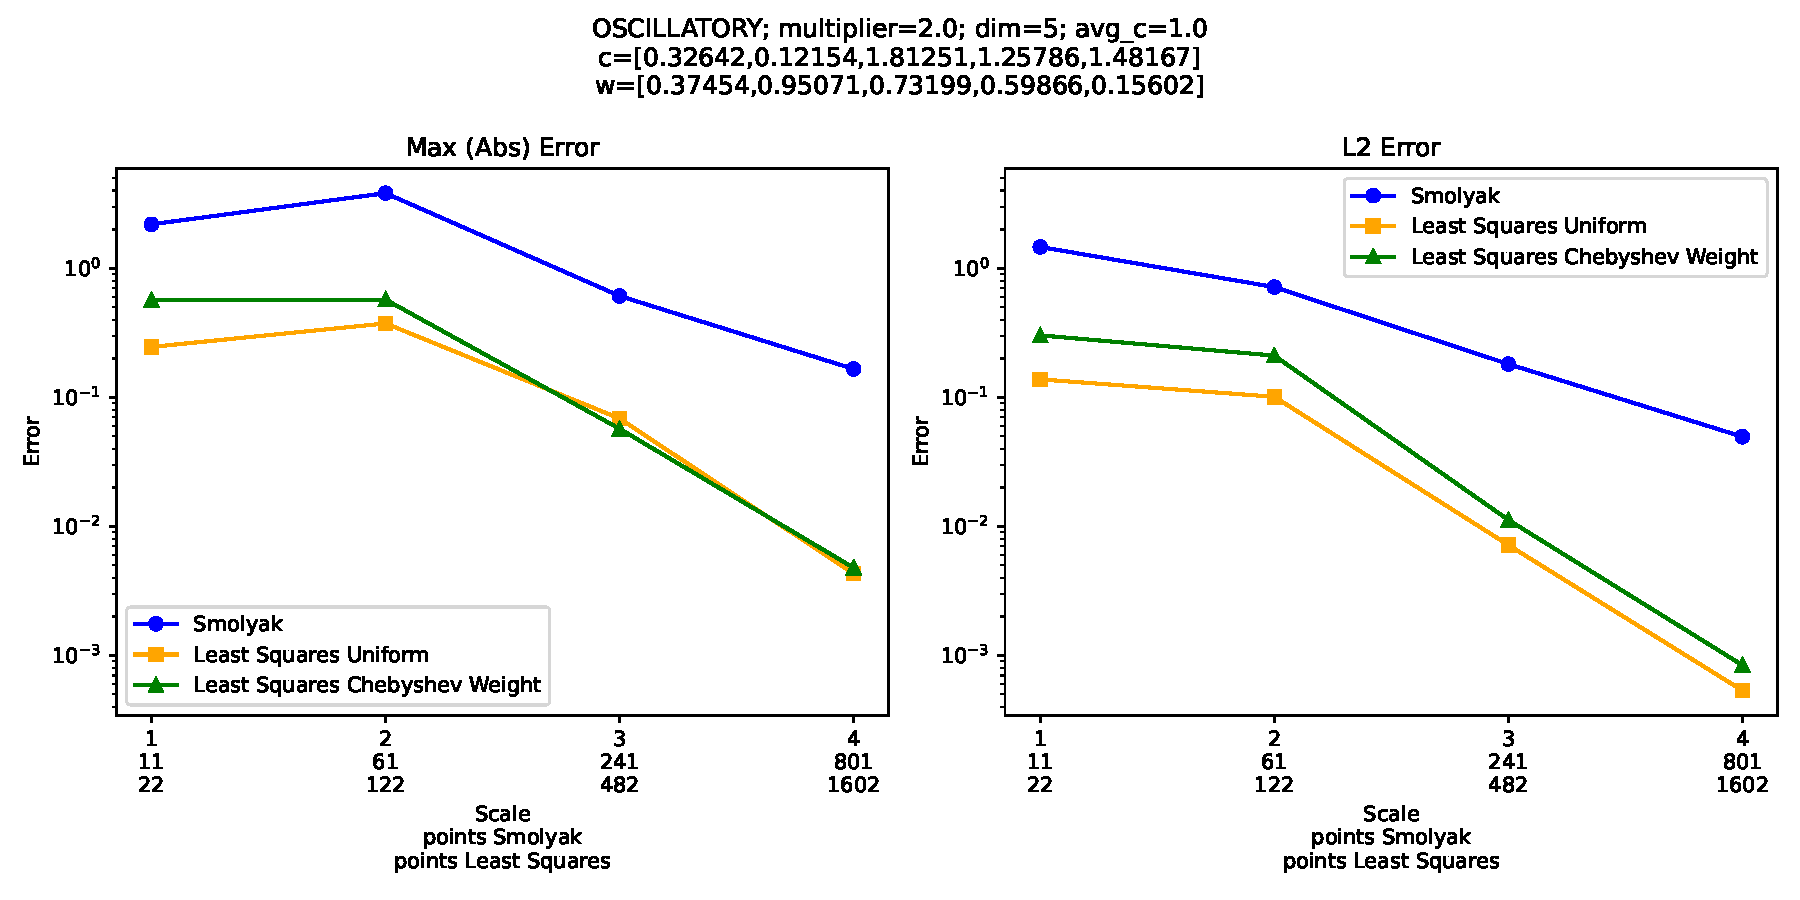
\includegraphics[width=\linewidth]{figures/oscillatory/realization1_dim5_scale4.pdf}
	\caption{Caption}
	\label{fig:Osc_1_dim5_scale4}
\end{figure}

\begin{figure}[H]
	\centering
	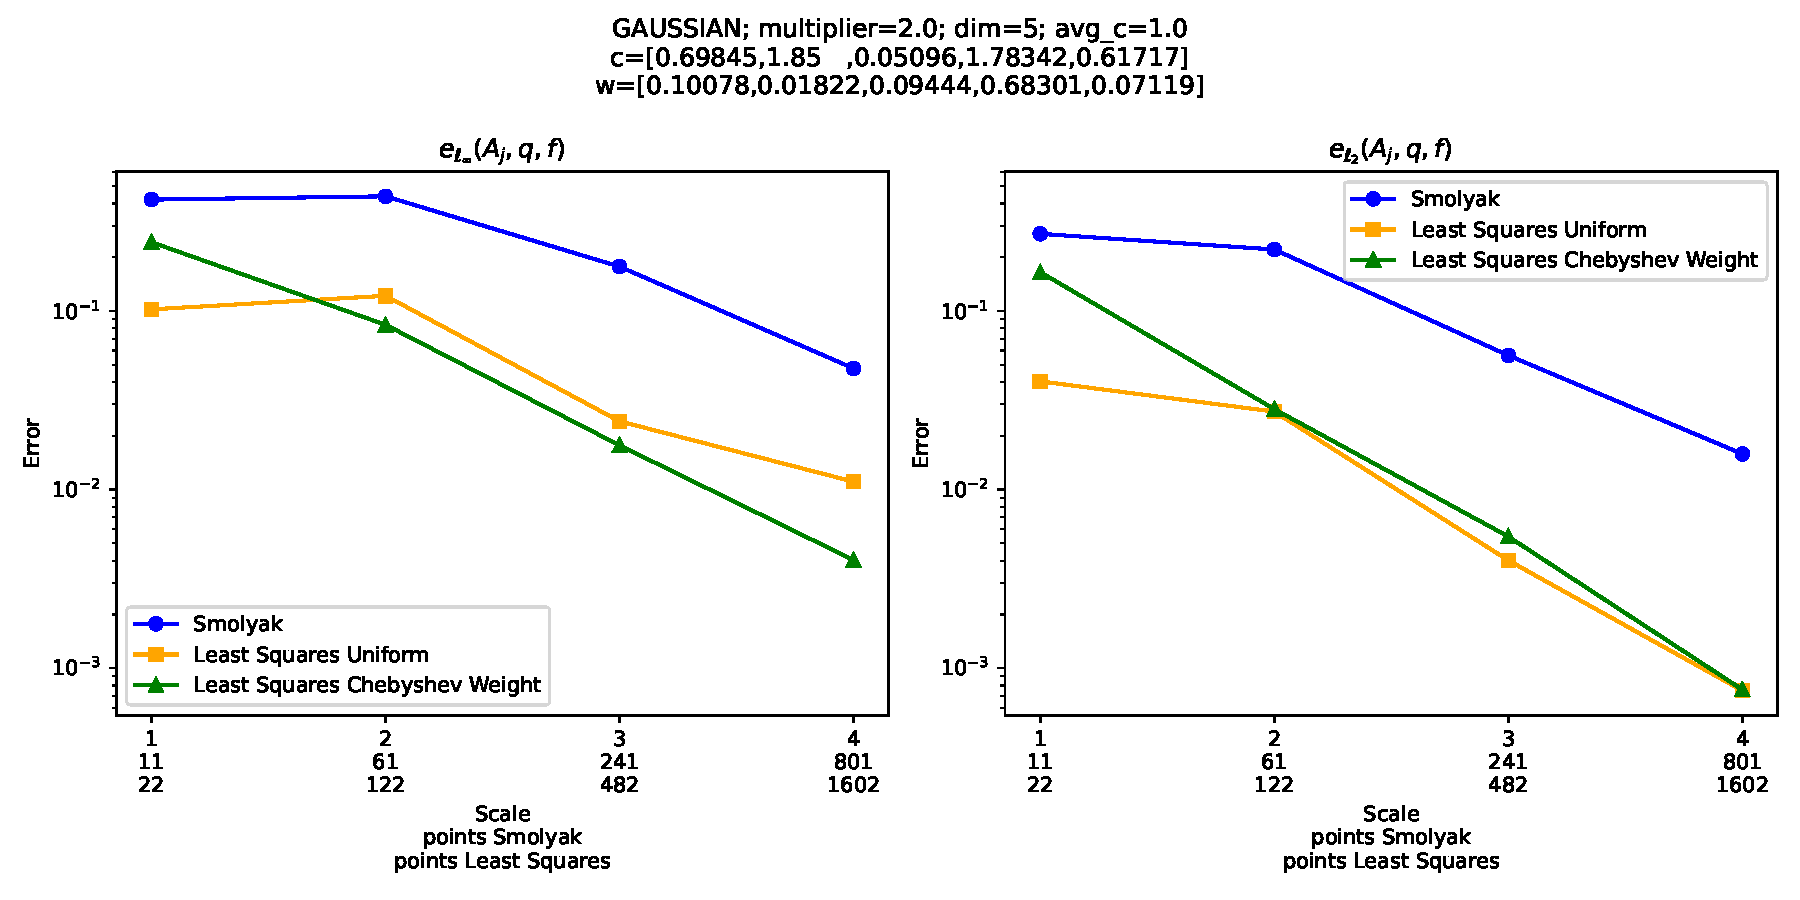
\includegraphics[width=\linewidth]{figures/oscillatory/realization2_dim5_scale4.pdf}
	\caption{Caption}
	\label{fig:Osc_2_dim5_scale4}
\end{figure}

\begin{figure}[H]
	\centering
	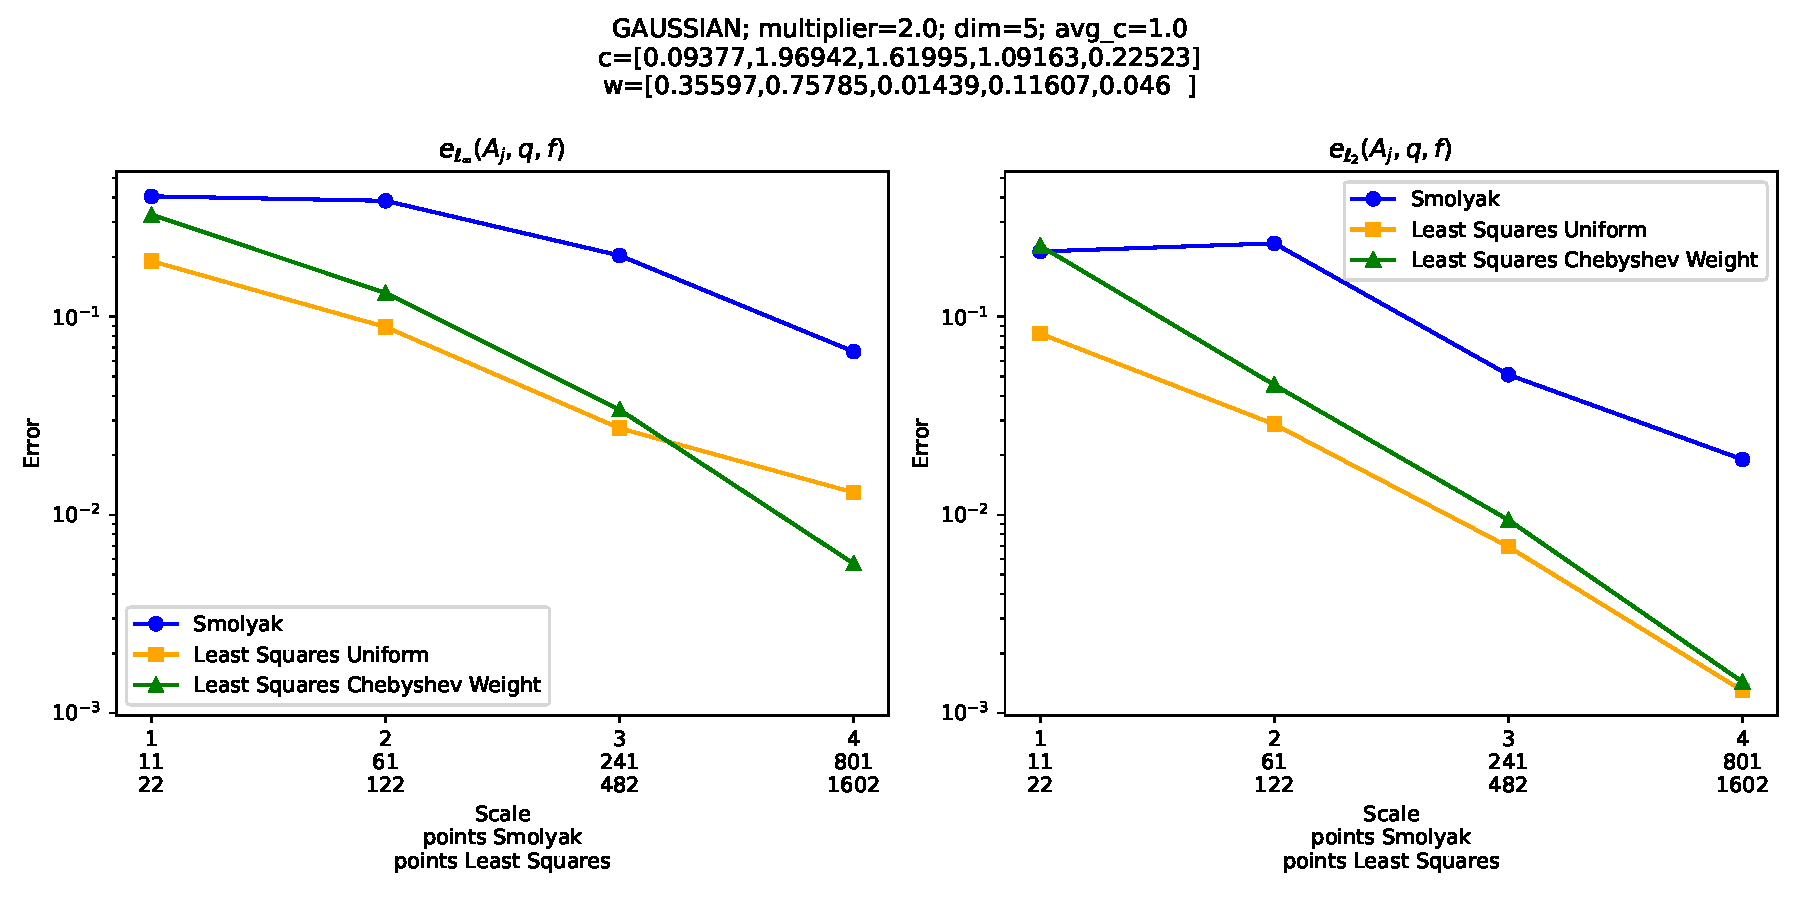
\includegraphics[width=\linewidth]{figures/oscillatory/realization3_dim5_scale4.pdf}
	\caption{Caption}
	\label{fig:Osc_3_dim5_scale4}
\end{figure}

\begin{figure}[H]
	\centering
	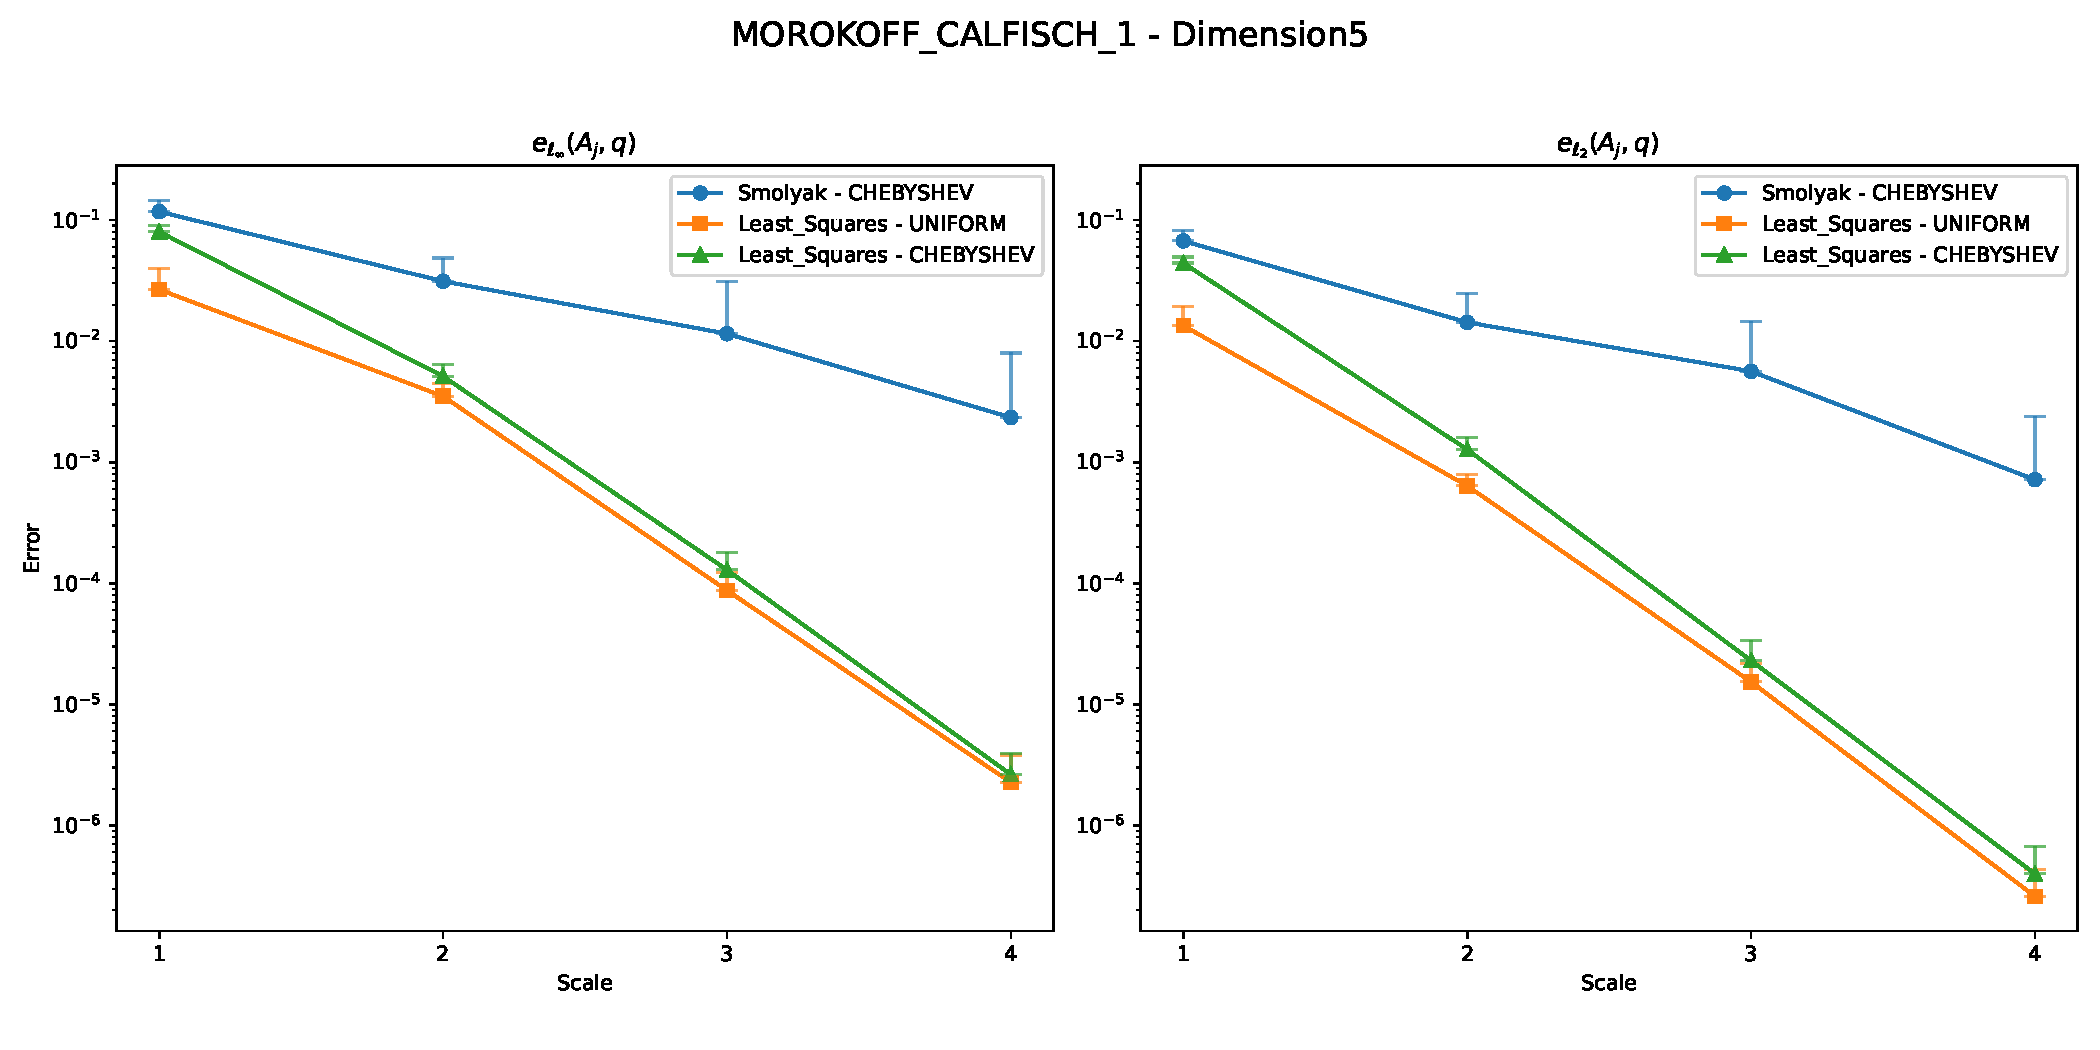
\includegraphics[width=\linewidth]{figures/morokoff_calfisch1/distro_dim5_scale4.pdf}
	\caption{Caption}
	\label{fig:morokoff_calfisch1_distribution_dim5_scale4}
\end{figure}

\begin{figure}[H]
	\centering
	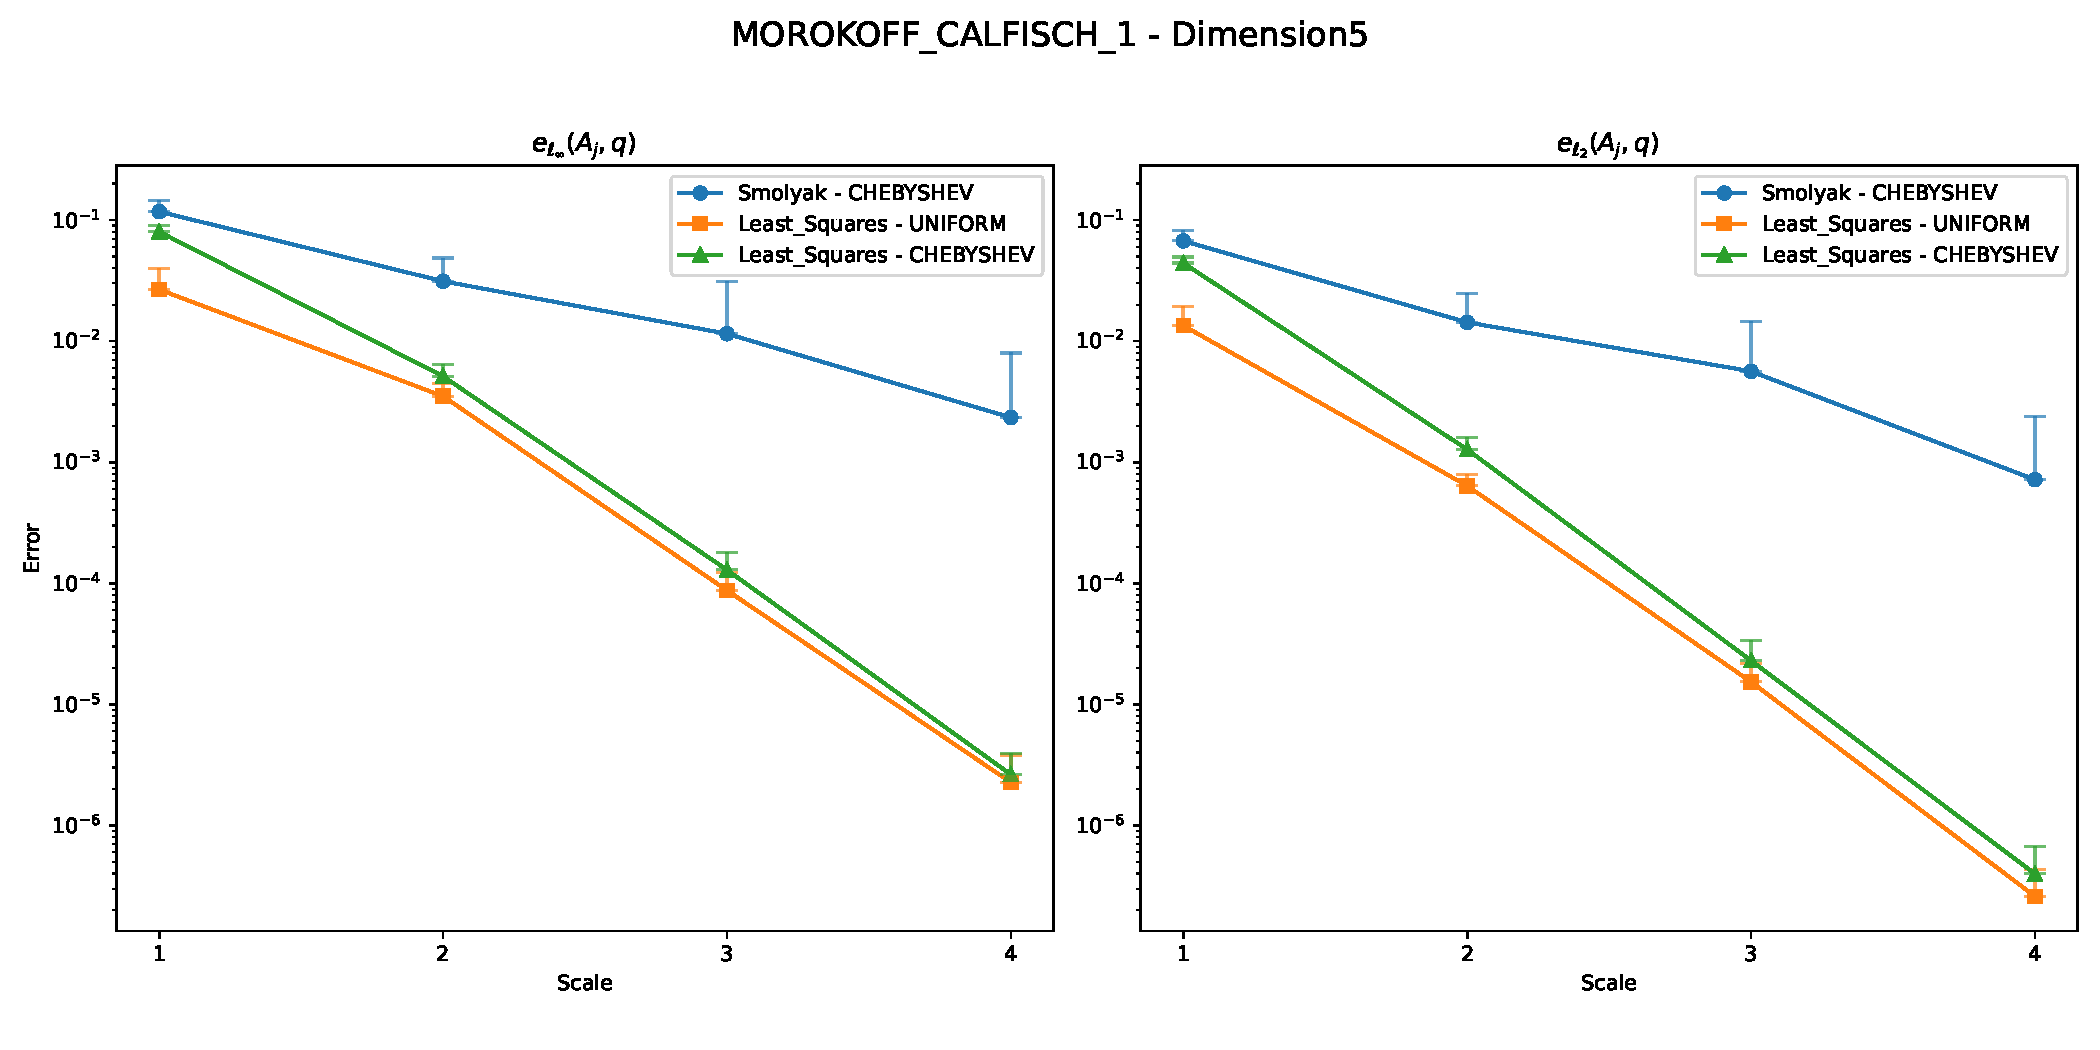
\includegraphics[width=\linewidth]{figures/morokoff_calfisch1/distro_dim5_scale4.pdf}
	\caption{Caption}
	\label{fig:morokoff_calfisch2_distribution_dim5_scale4}
\end{figure}

\begin{figure}[H] % TODO: Still with boxplot -> Maybe change
	\centering
	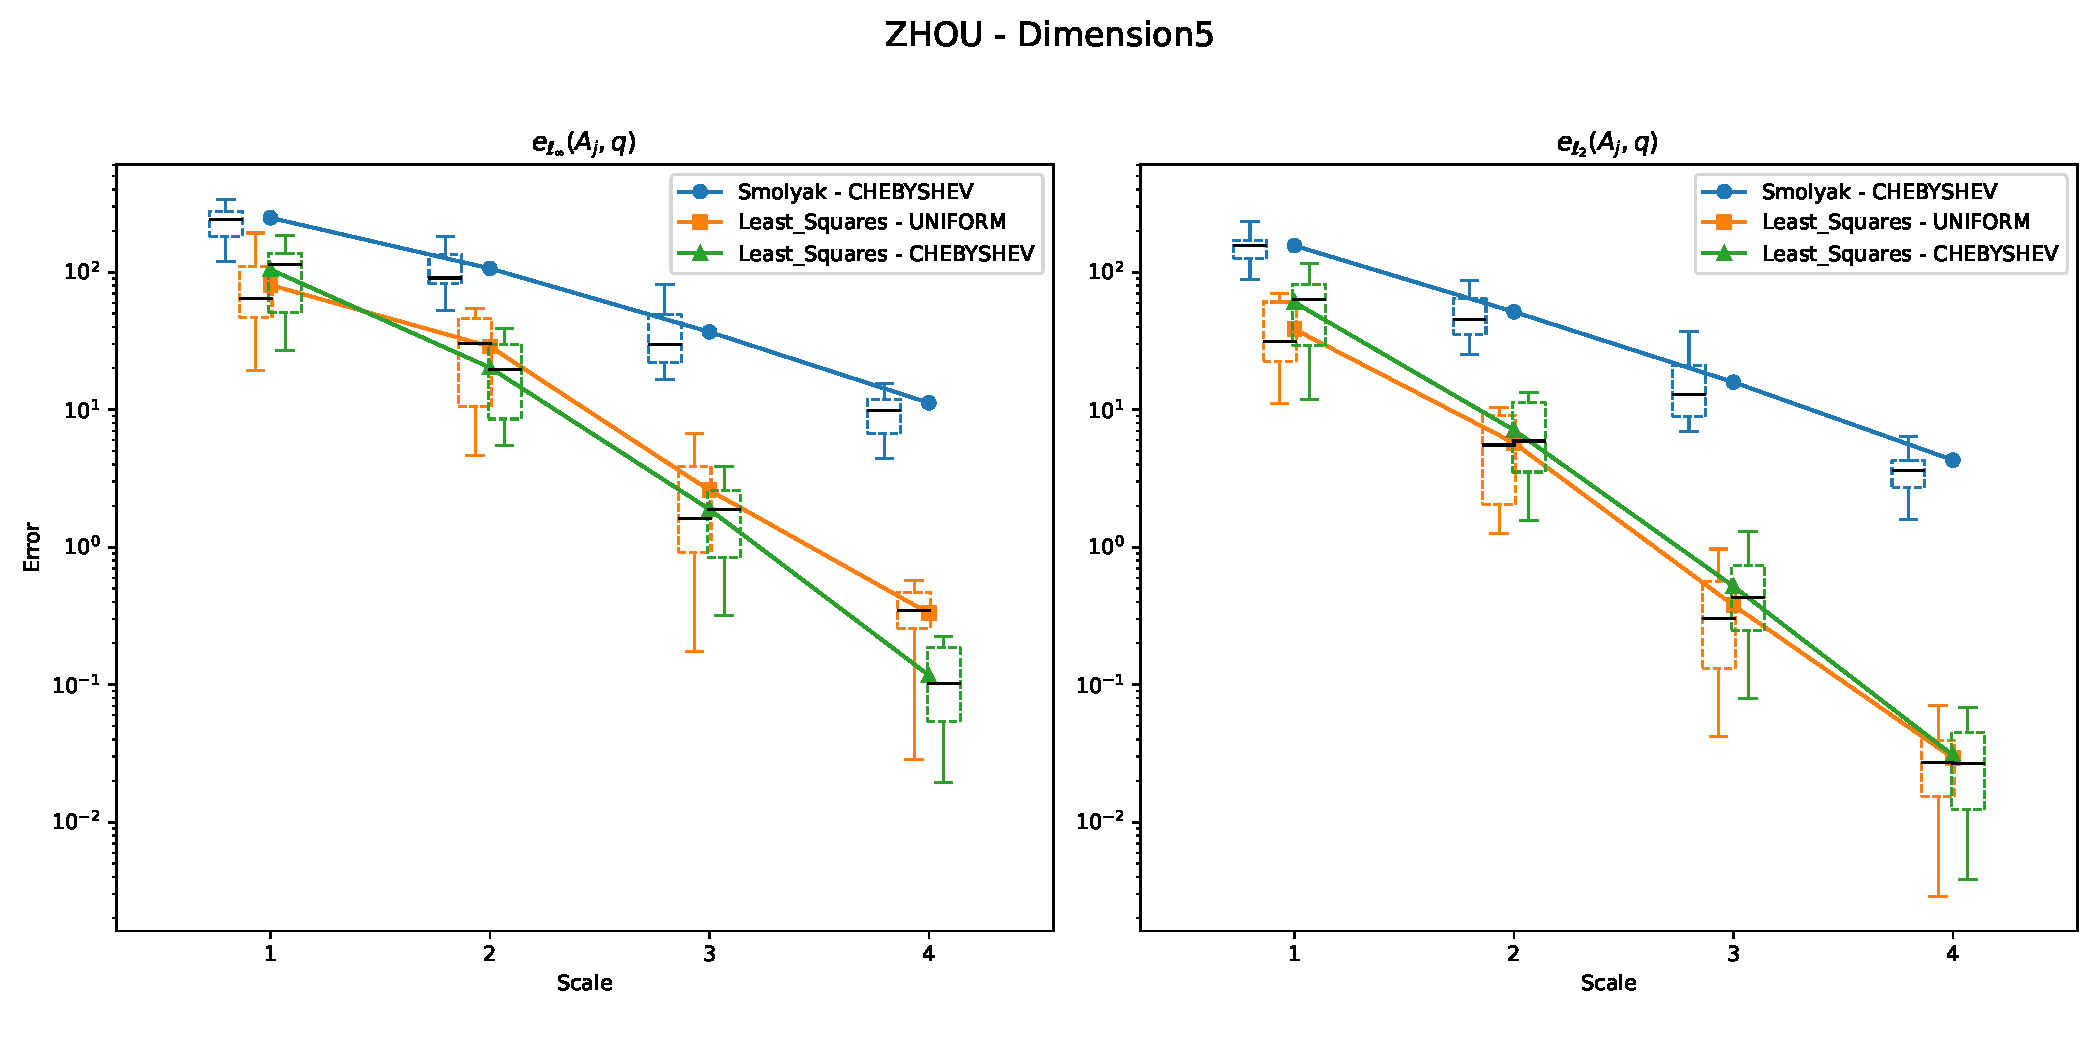
\includegraphics[width=\linewidth]{figures/zhou/distro_dim5_scale4.pdf}
	\caption{Caption}
	\label{fig:zhou_distribution_dim5_scale4}
\end{figure}

\begin{table}[H]
	\centering
	\begin{adjustbox}{width=\linewidth}
		% Created with Python on 2025-06-15 11:13:45
% ..\results\final_results\low_dim\results_numerical_experiments.csv, dim=2, scales = [3, 4, 5, 6, 7, 8, 9]
\begin{tabular}{ll|rr|rr|rr|rr|rr|rr|rr|}
 &   \multicolumn{1}{c}{} & \multicolumn{2}{c}{Scale 3} & \multicolumn{2}{c}{Scale 4} & \multicolumn{2}{c}{Scale 5} & \multicolumn{2}{c}{Scale 6} & \multicolumn{2}{c}{Scale 7} & \multicolumn{2}{c}{Scale 8} & \multicolumn{2}{c}{Scale 9}\\
 &   \multicolumn{1}{c}{} & \multicolumn{1}{c}{$e_{\rm max}^{\rm wc}$} & \multicolumn{1}{c}{$e_{\rm mean}^{\rm wc}$} & \multicolumn{1}{c}{$e_{\rm max}^{\rm wc}$} & \multicolumn{1}{c}{$e_{\rm mean}^{\rm wc}$} & \multicolumn{1}{c}{$e_{\rm max}^{\rm wc}$} & \multicolumn{1}{c}{$e_{\rm mean}^{\rm wc}$} & \multicolumn{1}{c}{$e_{\rm max}^{\rm wc}$} & \multicolumn{1}{c}{$e_{\rm mean}^{\rm wc}$} & \multicolumn{1}{c}{$e_{\rm max}^{\rm wc}$} & \multicolumn{1}{c}{$e_{\rm mean}^{\rm wc}$} & \multicolumn{1}{c}{$e_{\rm max}^{\rm wc}$} & \multicolumn{1}{c}{$e_{\rm mean}^{\rm wc}$} & \multicolumn{1}{c}{$e_{\rm max}^{\rm wc}$} & \multicolumn{1}{c}{$e_{\rm mean}^{\rm wc}$}\\
\toprule
\multirow{3}{*}{\thead[l]{\tiny\textbf{Bim. Gauss.}\\$Q=50$}} & Smolyak & \first{5.71e-01} & \first{2.69e-01}  & \first{3.66e-01} & 1.55e-01  & 1.91e-01 & 7.14e-02  & 3.33e-02 & 9.39e-03  & 2.47e-03 & 6.16e-04  & 8.96e-06 & 2.44e-06  & 7.95e-09 & 2.19e-09\\
 & LS-Uniform & 3.51e+00 & 8.16e-01  & 5.12e+00 & 7.82e-01  & 3.56e+00 & 3.27e-01  & 8.19e+00 & 7.13e-01  & 3.15e+02 & 1.41e+01  & 1.93e+00 & 6.95e-02  & 3.03e+04 & 5.31e+02\\
 & LS-Chebyshev & 7.40e-01 & 2.89e-01  & 4.20e-01 & \first{1.35e-01}  & \first{1.87e-01} & \first{4.82e-02}  & \first{2.24e-02} & \first{6.11e-03}  & \first{1.52e-03} & \first{4.10e-04}  & \first{6.78e-06} & \first{1.50e-06}  & \first{7.27e-09} & \first{1.52e-09}\\
\midrule
\multirow{3}{*}{\thead[l]{\tiny\textbf{Cont.}\\$Q=50$}} & Smolyak & \first{4.40e-02} & \first{1.49e-02}  & 2.22e-02 & 5.15e-03  & 1.10e-02 & 1.58e-03  & 5.23e-03 & 6.18e-04  & 2.68e-03 & 2.17e-04  & 1.46e-03 & 8.93e-05  & 7.65e-04 & 2.95e-05\\
 & LS-Uniform & 2.66e-01 & 7.08e-02  & 5.19e-01 & 7.51e-02  & 3.64e-01 & 3.24e-02  & 6.88e-01 & 6.27e-02  & 5.86e+02 & 2.69e+01  & 7.77e+02 & 3.19e+01  & 8.46e+08 & 1.50e+07\\
 & LS-Chebyshev & 4.80e-02 & 2.21e-02  & \first{1.84e-02} & \first{4.06e-03}  & \first{9.43e-03} & \first{1.45e-03}  & \first{4.69e-03} & \first{4.91e-04}  & \first{2.08e-03} & \first{1.85e-04}  & \first{1.20e-03} & \first{6.72e-05}  & \first{6.47e-04} & \first{2.71e-05}\\
\midrule
\multirow{3}{*}{\thead[l]{\tiny\textbf{Corner Peak}\\$Q=50$}} & Smolyak & \first{8.78e-03} & 4.52e-03  & 1.48e-03 & 5.81e-04  & 1.04e-04 & 3.31e-05  & 8.90e-07 & 2.61e-07  & \first{6.08e-09} & 1.75e-09  & \first{2.77e-13} & 8.54e-14  & \first{6.99e-15} & \first{9.35e-16}\\
 & LS-Uniform & 1.54e-02 & 3.24e-03  & 3.50e-03 & 5.50e-04  & 4.92e-04 & 5.98e-05  & 2.30e-04 & 2.04e-05  & 6.80e-04 & 3.05e-05  & 7.93e-08 & 2.70e-09  & 1.66e-02 & 2.92e-04\\
 & LS-Chebyshev & 8.88e-03 & \first{3.12e-03}  & \first{1.42e-03} & \first{4.44e-04}  & \first{8.77e-05} & \first{2.65e-05}  & \first{6.13e-07} & \first{1.70e-07}  & 6.32e-09 & \first{1.30e-09}  & 2.79e-13 & \first{5.98e-14}  & 1.39e-14 & 1.17e-15\\
\midrule
\multirow{3}{*}{\thead[l]{\tiny\textbf{Discont.}\\$Q=50$}} & Smolyak & 4.73e+00 & \first{1.26e+00}  & 3.82e+00 & 1.08e+00  & 4.82e+00 & 8.42e-01  & 4.56e+00 & 6.75e-01  & 4.07e+00 & 4.26e-01  & 3.57e+00 & 3.28e-01  & 4.70e+00 & 2.16e-01\\
 & LS-Uniform & 3.46e+01 & 8.99e+00  & 7.48e+01 & 1.09e+01  & 6.02e+01 & 6.33e+00  & 3.07e+02 & 2.72e+01  & 6.62e+05 & 2.77e+04  & 1.79e+06 & 6.20e+04  & 6.27e+12 & 1.10e+11\\
 & LS-Chebyshev & \first{3.47e+00} & 1.27e+00  & \first{3.59e+00} & \first{7.15e-01}  & \first{4.24e+00} & \first{6.58e-01}  & \first{3.44e+00} & \first{4.35e-01}  & \first{3.25e+00} & \first{2.92e-01}  & \first{2.36e+00} & \first{2.04e-01}  & \first{2.92e+00} & \first{1.46e-01}\\
\midrule
\multirow{3}{*}{\thead[l]{\tiny\textbf{Gauss.}\\$Q=50$}} & Smolyak & 5.81e-01 & 2.39e-01  & 3.51e-01 & 9.72e-02  & 1.18e-01 & 3.11e-02  & 2.17e-02 & 5.03e-03  & 1.93e-03 & 4.27e-04  & 7.40e-06 & 1.88e-06  & 6.31e-09 & 1.51e-09\\
 & LS-Uniform & 3.13e+00 & 7.97e-01  & 3.83e+00 & 5.77e-01  & 3.44e+00 & 2.92e-01  & 7.53e+00 & 6.71e-01  & 2.27e+02 & 1.11e+01  & 2.62e+00 & 8.97e-02  & 1.88e+04 & 3.30e+02\\
 & LS-Chebyshev & \first{4.84e-01} & \first{1.75e-01}  & \first{3.40e-01} & \first{8.12e-02}  & \first{6.74e-02} & \first{1.90e-02}  & \first{1.67e-02} & \first{3.37e-03}  & \first{1.19e-03} & \first{2.87e-04}  & \first{5.39e-06} & \first{1.22e-06}  & \first{5.51e-09} & \first{1.08e-09}\\
\midrule
\multirow{3}{*}{\thead[l]{\tiny\textbf{Geo. Mean}\\$Q=50$}} & Smolyak & 1.09e-02 & 5.50e-03  & 2.80e-03 & \first{7.19e-04}  & \first{3.70e-04} & \first{7.25e-05}  & 4.84e-05 & 8.72e-06  & 3.65e-06 & 6.94e-07  & 1.36e-07 & 2.22e-08  & 2.19e-09 & 3.61e-10\\
 & LS-Uniform & \first{7.18e-03} & \first{1.52e-03}  & 5.70e-03 & 1.08e-03  & 1.33e-03 & 1.36e-04  & 3.29e-03 & 2.95e-04  & 1.07e-01 & 4.54e-03  & 3.88e-03 & 1.23e-04  & 2.26e+02 & 3.95e+00\\
 & LS-Chebyshev & 9.32e-03 & 4.52e-03  & \first{2.45e-03} & 9.90e-04  & 5.63e-04 & 9.85e-05  & \first{3.23e-05} & \first{7.11e-06}  & \first{3.08e-06} & \first{5.99e-07}  & \first{9.87e-08} & \first{2.00e-08}  & \first{2.06e-09} & \first{3.03e-10}\\
\midrule
\multirow{3}{*}{\thead[l]{\tiny\textbf{NOISE}\\$Q=50$}} & Smolyak & 6.00e-07 & 3.07e-07  & 6.46e-07 & 2.64e-07  & 7.78e-07 & 2.43e-07  & \first{8.85e-07} & 2.38e-07  & 9.21e-07 & 2.39e-07  & 1.21e-06 & 2.51e-07  & 1.25e-06 & 2.57e-07\\
 & LS-Uniform & 4.11e-06 & 1.04e-06  & 2.12e-05 & 3.07e-06  & 1.98e-05 & 2.30e-06  & 2.21e-04 & 2.00e-05  & 5.97e-01 & 2.69e-02  & 1.65e+00 & 5.52e-02  & 1.05e+07 & 1.84e+05\\
 & LS-Chebyshev & \first{5.59e-07} & \first{2.36e-07}  & \first{5.80e-07} & \first{1.97e-07}  & \first{7.30e-07} & \first{1.51e-07}  & 1.13e-06 & \first{1.47e-07}  & \first{8.96e-07} & \first{1.35e-07}  & \first{7.56e-07} & \first{1.28e-07}  & \first{7.61e-07} & \first{1.27e-07}\\
\midrule
\multirow{3}{*}{\thead[l]{\tiny\textbf{Osci.}\\$Q=50$}} & Smolyak & \first{3.97e-02} & 2.52e-02  & \first{2.12e-03} & 1.06e-03  & \first{4.48e-05} & 1.87e-05  & 9.42e-09 & 3.35e-09  & 5.70e-13 & 1.95e-13  & \first{9.44e-15} & \first{2.26e-15}  & \first{1.97e-14} & 3.65e-15\\
 & LS-Uniform & 1.69e-01 & 3.71e-02  & 9.31e-03 & 1.42e-03  & 1.97e-04 & 3.00e-05  & 2.71e-06 & 2.40e-07  & 7.01e-08 & 3.60e-09  & 7.54e-09 & 2.53e-10  & 5.83e-02 & 1.02e-03\\
 & LS-Chebyshev & 4.57e-02 & \first{1.78e-02}  & 2.53e-03 & \first{8.35e-04}  & 5.56e-05 & \first{1.33e-05}  & \first{7.69e-09} & \first{2.20e-09}  & \first{5.26e-13} & \first{1.40e-13}  & 3.43e-14 & 2.88e-15  & 2.81e-14 & \first{2.41e-15}\\
\midrule
\multirow{3}{*}{\thead[l]{\tiny\textbf{Prod. Peak}\\$Q=50$}} & Smolyak & \first{1.04e-03} & 6.17e-04  & \first{8.63e-05} & 3.77e-05  & 3.51e-06 & 1.24e-06  & 2.27e-08 & 7.41e-09  & 3.03e-11 & 8.55e-12  & \first{7.77e-15} & 2.15e-15  & \first{1.80e-14} & 3.63e-15\\
 & LS-Uniform & 4.27e-03 & 9.86e-04  & 4.65e-04 & 7.06e-05  & 1.99e-05 & 2.55e-06  & 7.28e-06 & 6.43e-07  & 3.65e-06 & 1.54e-07  & 3.19e-09 & 1.14e-10  & 2.16e-02 & 3.83e-04\\
 & LS-Chebyshev & 1.05e-03 & \first{5.03e-04}  & 1.01e-04 & \first{3.20e-05}  & \first{3.45e-06} & \first{8.70e-07}  & \first{1.81e-08} & \first{4.66e-09}  & \first{2.75e-11} & \first{6.14e-12}  & 1.55e-14 & \first{1.79e-15}  & 2.56e-14 & \first{1.73e-15}\\
\midrule
\multirow{3}{*}{\thead[l]{\tiny\textbf{Ridge Prod.}\\$Q=50$}} & Smolyak & 2.48e-01 & 1.05e-01  & \first{1.14e-01} & \first{3.85e-02}  & \first{6.89e-02} & 1.54e-02  & \first{3.42e-02} & 5.39e-03  & \first{2.39e-02} & 2.13e-03  & 1.18e-02 & 9.11e-04  & 7.14e-03 & 3.33e-04\\
 & LS-Uniform & 1.29e+00 & 3.18e-01  & 2.37e+00 & 3.45e-01  & 1.61e+00 & 1.67e-01  & 9.01e+00 & 7.85e-01  & 6.36e+03 & 2.86e+02  & 5.10e+03 & 1.54e+02  & 1.57e+10 & 2.75e+08\\
 & LS-Chebyshev & \first{1.94e-01} & \first{6.80e-02}  & 1.17e-01 & 4.08e-02  & 8.27e-02 & \first{1.14e-02}  & 4.75e-02 & \first{4.39e-03}  & 2.72e-02 & \first{1.68e-03}  & \first{1.14e-02} & \first{6.19e-04}  & \first{5.41e-03} & \first{2.38e-04}\\
\bottomrule
\end{tabular}

	\end{adjustbox}
	\caption{Caption}
	\label{tab:dim2_results}
\end{table}

\begin{table}[H]
	\centering
	\begin{adjustbox}{width=\linewidth}
		% Created with Python on 2025-04-21 15:33:59
% C:\Users\jakob\Documents\Repos\NumericalExperiments\results\combined_results_numerical_experiments.csv, scale=3, dims = [2, 3, 4, 5, 6, 7, 8, 9, 10]
\begin{tabular}{ll|rr|rr|rr|rr|rr|rr|rr|rr|rr|}
 &   \multicolumn{1}{c}{} & \multicolumn{2}{c}{Dim2} & \multicolumn{2}{c}{Dim3} & \multicolumn{2}{c}{Dim4} & \multicolumn{2}{c}{Dim5} & \multicolumn{2}{c}{Dim6} & \multicolumn{2}{c}{Dim7} & \multicolumn{2}{c}{Dim8} & \multicolumn{2}{c}{Dim9} & \multicolumn{2}{c}{Dim10}\\
 &   \multicolumn{1}{c}{} & \multicolumn{2}{c}{max} & \multicolumn{2}{c}{max} & \multicolumn{2}{c}{max} & \multicolumn{2}{c}{max} & \multicolumn{2}{c}{max} & \multicolumn{2}{c}{max} & \multicolumn{2}{c}{max} & \multicolumn{2}{c}{max} & \multicolumn{2}{c}{max}\\
 &   \multicolumn{1}{c}{} & \multicolumn{1}{c}{$\ell_2$} & \multicolumn{1}{c}{$\ell_\infty$} & \multicolumn{1}{c}{$\ell_2$} & \multicolumn{1}{c}{$\ell_\infty$} & \multicolumn{1}{c}{$\ell_2$} & \multicolumn{1}{c}{$\ell_\infty$} & \multicolumn{1}{c}{$\ell_2$} & \multicolumn{1}{c}{$\ell_\infty$} & \multicolumn{1}{c}{$\ell_2$} & \multicolumn{1}{c}{$\ell_\infty$} & \multicolumn{1}{c}{$\ell_2$} & \multicolumn{1}{c}{$\ell_\infty$} & \multicolumn{1}{c}{$\ell_2$} & \multicolumn{1}{c}{$\ell_\infty$} & \multicolumn{1}{c}{$\ell_2$} & \multicolumn{1}{c}{$\ell_\infty$} & \multicolumn{1}{c}{$\ell_2$} & \multicolumn{1}{c}{$\ell_\infty$}\\
\toprule
\multirow{3}{*}{\thead[l]{\tiny\textbf{Bratley}\\$n=10$}} & Smolyak & \first{6.27e-16} & \first{1.33e-15}  & \first{7.02e-16} & \first{2.22e-15}  & \first{5.29e-03} & \first{2.57e-02}  & \first{2.57e-02} & \first{1.58e-01}  & \first{1.62e-02} & \first{1.00e-01}  & \first{2.53e-02} & \first{2.08e-01}  & \first{2.45e-02} & 2.73e-01  & \first{4.45e-02} & \first{2.98e-01}  & \first{2.69e-02} & \first{3.25e-01}\\
 & LS-Uniform & 1.11e-15 & 3.55e-15  & 1.97e-15 & 7.33e-15  & 1.20e-02 & 6.85e-02  & 3.97e-02 & 2.41e-01  & 2.41e-02 & 1.67e-01  & 4.17e-02 & 3.51e-01  & 3.58e-02 & \first{2.27e-01}  & 6.53e-02 & 4.35e-01  & 4.14e-02 & 3.51e-01\\
 & LS-Chebyshev & 2.45e-15 & 7.11e-15  & 1.84e-15 & 5.55e-15  & 1.95e-02 & 6.84e-02  & 8.66e-02 & 4.19e-01  & 6.27e-02 & 2.18e-01  & 7.72e-02 & 3.80e-01  & 6.60e-02 & 4.70e-01  & 1.83e-01 & 6.48e-01  & 9.14e-02 & 3.80e-01\\
\midrule
\multirow{3}{*}{\thead[l]{\tiny\textbf{Continuous}\\$n=10$}} & Smolyak & 2.50e-02 & 9.26e-02  & 2.87e-02 & \first{8.67e-02}  & 3.75e-02 & \first{1.16e-01}  & 2.96e-02 & 1.53e-01  & 5.04e-02 & 1.57e-01  & 3.58e-02 & 1.76e-01  & 2.08e-02 & 2.16e-01  & 3.09e-02 & 2.10e-01  & 1.69e-02 & \first{1.22e-01}\\
 & LS-Uniform & 7.79e-02 & 2.84e-01  & 5.12e-02 & 2.39e-01  & 2.70e-02 & 1.37e-01  & 2.95e-02 & 1.59e-01  & 2.27e-02 & \first{1.49e-01}  & \first{1.53e-02} & \first{1.51e-01}  & \first{1.62e-02} & \first{1.42e-01}  & \first{1.44e-02} & \first{1.87e-01}  & \first{9.44e-03} & 1.24e-01\\
 & LS-Chebyshev & \first{1.90e-02} & \first{6.58e-02}  & \first{1.86e-02} & 9.44e-02  & \first{2.42e-02} & 1.19e-01  & \first{2.46e-02} & \first{1.42e-01}  & \first{2.12e-02} & 2.17e-01  & 1.72e-02 & 2.01e-01  & 1.62e-02 & 1.92e-01  & 1.75e-02 & 2.30e-01  & 1.06e-02 & 1.99e-01\\
\midrule
\multirow{3}{*}{\thead[l]{\tiny\textbf{Corner Peak}\\$n=10$}} & Smolyak & 4.52e-03 & 8.68e-03  & 1.36e-02 & 5.59e-02  & 2.22e-02 & 1.64e-01  & 1.14e-02 & 8.92e-02  & 2.81e-03 & \first{2.15e-02}  & 9.43e-04 & 2.78e-02  & \first{1.91e-05} & \first{6.36e-04}  & \first{9.96e-06} & 3.36e-04  & \first{4.22e-07} & 2.15e-05\\
 & LS-Uniform & 3.23e-03 & 1.54e-02  & 1.20e-02 & 5.84e-02  & \first{9.98e-03} & \first{7.21e-02}  & \first{3.14e-03} & \first{2.87e-02}  & \first{2.71e-03} & 2.87e-02  & \first{8.01e-04} & \first{2.66e-02}  & 1.42e-04 & 2.31e-03  & 1.12e-05 & \first{2.87e-04}  & 8.78e-07 & \first{1.96e-05}\\
 & LS-Chebyshev & \first{2.62e-03} & \first{8.10e-03}  & \first{1.12e-02} & \first{3.55e-02}  & 3.67e-02 & 1.08e-01  & 3.22e-02 & 1.49e-01  & 6.43e-03 & 2.22e-02  & 1.08e-03 & 2.77e-02  & 2.30e-04 & 1.76e-03  & 3.54e-04 & 1.29e-03  & 2.43e-06 & 2.02e-05\\
\midrule
\multirow{3}{*}{\thead[l]{\tiny\textbf{Discontinuous}\\$n=10$}} & Smolyak & 1.12e+00 & \first{2.83e+00}  & 2.55e+00 & 8.43e+00  & 5.20e+00 & 2.15e+01  & 7.04e+00 & 4.40e+01  & \first{1.22e+01} & 1.32e+02  & \first{2.31e+01} & 3.28e+02  & 3.23e+01 & \first{4.10e+02}  & \first{7.13e+01} & 8.03e+02  & \first{1.08e+02} & 2.13e+03\\
 & LS-Uniform & 2.65e+00 & 1.07e+01  & 4.14e+00 & 1.59e+01  & 4.30e+00 & 2.31e+01  & \first{6.97e+00} & 4.17e+01  & 1.38e+01 & 1.21e+02  & 2.80e+01 & \first{2.17e+02}  & \first{3.13e+01} & 4.57e+02  & 8.33e+01 & \first{6.98e+02}  & 1.10e+02 & \first{1.17e+03}\\
 & LS-Chebyshev & \first{1.06e+00} & 4.16e+00  & \first{2.36e+00} & \first{7.11e+00}  & \first{3.35e+00} & \first{1.27e+01}  & 8.53e+00 & \first{3.01e+01}  & 1.65e+01 & \first{9.97e+01}  & 5.05e+01 & 3.24e+02  & 5.35e+01 & 4.26e+02  & 1.30e+02 & 1.36e+03  & 3.68e+02 & 1.80e+03\\
\midrule
\multirow{3}{*}{\thead[l]{\tiny\textbf{Gaussian}\\$n=10$}} & Smolyak & 5.85e-04 & 8.95e-04  & 3.93e-03 & 7.46e-03  & 5.19e-03 & 1.50e-02  & 1.10e-02 & 3.39e-02  & 1.03e-02 & \first{4.42e-02}  & 2.04e-02 & 8.19e-02  & 1.66e-02 & \first{9.36e-02}  & 2.33e-02 & 1.87e-01  & \first{1.44e-02} & \first{1.40e-01}\\
 & LS-Uniform & 8.71e-04 & 3.82e-03  & 3.91e-03 & 2.16e-02  & \first{3.68e-03} & 3.06e-02  & \first{7.90e-03} & 5.69e-02  & \first{8.16e-03} & 6.35e-02  & \first{1.43e-02} & 1.76e-01  & \first{1.65e-02} & 1.85e-01  & \first{1.60e-02} & 1.54e-01  & 1.64e-02 & 2.23e-01\\
 & LS-Chebyshev & \first{2.86e-04} & \first{7.18e-04}  & \first{2.53e-03} & \first{6.34e-03}  & 4.39e-03 & \first{1.24e-02}  & 1.05e-02 & \first{3.20e-02}  & 1.41e-02 & 5.01e-02  & 1.97e-02 & \first{7.26e-02}  & 2.39e-02 & 1.51e-01  & 2.57e-02 & \first{1.37e-01}  & 2.47e-02 & 1.93e-01\\
\midrule
\multirow{3}{*}{\thead[l]{\tiny\textbf{G-Function}\\$n=10$}} & Smolyak & 8.16e-02 & 2.13e-01  & 1.99e-01 & 6.79e-01  & 3.74e-01 & 1.35e+00  & 6.12e-01 & 3.56e+00  & 7.87e-01 & 6.08e+00  & 1.33e+00 & 1.92e+01  & 1.49e+00 & 2.39e+01  & 1.94e+00 & 2.43e+01  & 3.36e+00 & 5.23e+01\\
 & LS-Uniform & 3.64e-01 & 1.48e+00  & 1.97e-01 & 9.60e-01  & \first{3.74e-01} & 2.64e+00  & \first{3.88e-01} & 2.37e+00  & \first{6.38e-01} & 3.14e+00  & \first{6.32e-01} & \first{4.80e+00}  & \first{8.08e-01} & \first{7.67e+00}  & \first{1.00e+00} & \first{1.02e+01}  & \first{1.42e+00} & 1.81e+01\\
 & LS-Chebyshev & \first{6.08e-02} & \first{1.44e-01}  & \first{1.45e-01} & \first{4.01e-01}  & 3.90e-01 & \first{1.27e+00}  & 4.79e-01 & \first{2.14e+00}  & 8.05e-01 & \first{2.95e+00}  & 7.16e-01 & 4.88e+00  & 1.08e+00 & 9.30e+00  & 3.21e+00 & 1.22e+01  & 3.07e+00 & \first{1.80e+01}\\
\midrule
\multirow{3}{*}{\thead[l]{\tiny\textbf{Morokoff Calfisch 1}\\$n=10$}} & Smolyak & 1.66e-03 & 3.21e-03  & \first{2.84e-03} & \first{9.40e-03}  & 2.37e-02 & 9.16e-02  & 3.19e-02 & 1.27e-01  & 3.12e-02 & 1.70e-01  & 1.01e-02 & 4.78e-02  & 2.75e-03 & 2.04e-02  & 2.87e-02 & 1.44e-01  & 1.91e-02 & 9.96e-02\\
 & LS-Uniform & \first{4.82e-04} & \first{1.93e-03}  & 4.34e-03 & 2.23e-02  & \first{1.37e-02} & 1.38e-01  & \first{1.75e-02} & 1.38e-01  & \first{1.25e-02} & \first{1.02e-01}  & \first{5.38e-03} & 6.23e-02  & \first{1.54e-03} & 2.05e-02  & \first{1.33e-02} & \first{1.13e-01}  & \first{9.92e-03} & 9.09e-02\\
 & LS-Chebyshev & 1.82e-03 & 3.73e-03  & 4.37e-03 & 1.58e-02  & 2.67e-02 & \first{8.95e-02}  & 3.34e-02 & \first{1.18e-01}  & 2.80e-02 & 1.40e-01  & 8.74e-03 & \first{4.46e-02}  & 2.39e-03 & \first{1.12e-02}  & 3.69e-02 & 1.32e-01  & 1.73e-02 & \first{7.04e-02}\\
\midrule
\multirow{3}{*}{\thead[l]{\tiny\textbf{Morokoff Calfisch 2}\\$n=10$}} & Smolyak & \first{7.91e-16} & \first{1.78e-15}  & \first{1.36e-15} & \first{4.44e-15}  & \first{3.39e-05} & \first{1.65e-04}  & \first{4.04e-05} & \first{2.20e-04}  & \first{4.23e-05} & \first{3.38e-04}  & \first{2.48e-05} & \first{3.31e-04}  & \first{2.04e-05} & \first{1.53e-04}  & \first{3.03e-05} & \first{3.66e-04}  & \first{2.32e-05} & 3.25e-04\\
 & LS-Uniform & 1.93e-15 & 7.11e-15  & 4.91e-15 & 1.87e-14  & 7.70e-05 & 4.40e-04  & 7.14e-05 & 3.32e-04  & 6.84e-05 & 4.06e-04  & 3.76e-05 & 6.02e-04  & 3.30e-05 & 2.58e-04  & 4.88e-05 & 3.83e-04  & 3.59e-05 & \first{3.17e-04}\\
 & LS-Chebyshev & 5.53e-15 & 1.47e-14  & 2.91e-15 & 6.66e-15  & 1.25e-04 & 4.39e-04  & 1.61e-04 & 5.52e-04  & 1.74e-04 & 5.79e-04  & 6.60e-05 & 9.22e-04  & 6.37e-05 & 4.61e-04  & 1.32e-04 & 6.62e-04  & 7.10e-05 & 5.42e-04\\
\midrule
\multirow{3}{*}{\thead[l]{\tiny\textbf{Oscillatory}\\$n=10$}} & Smolyak & 4.66e-05 & \first{7.06e-05}  & 1.16e-03 & \first{2.69e-03}  & \first{4.20e-03} & \first{2.17e-02}  & \first{1.11e-02} & \first{6.58e-02}  & \first{2.11e-02} & \first{1.86e-01}  & \first{3.83e-02} & \first{4.20e-01}  & \first{4.33e-02} & \first{4.17e-01}  & \first{7.70e-02} & 1.09e+00  & \first{9.24e-02} & 2.42e+00\\
 & LS-Uniform & 5.94e-05 & 2.74e-04  & 1.21e-03 & 5.95e-03  & 8.49e-03 & 4.88e-02  & 1.97e-02 & 1.07e-01  & 3.77e-02 & 2.85e-01  & 5.51e-02 & 6.55e-01  & 6.82e-02 & 5.12e-01  & 1.18e-01 & \first{1.08e+00}  & 1.33e-01 & \first{1.45e+00}\\
 & LS-Chebyshev & \first{2.43e-05} & 7.37e-05  & \first{1.03e-03} & 2.84e-03  & 1.29e-02 & 4.68e-02  & 4.24e-02 & 1.44e-01  & 7.57e-02 & 2.97e-01  & 9.50e-02 & 9.65e-01  & 1.01e-01 & 7.33e-01  & 2.71e-01 & 1.14e+00  & 2.16e-01 & 1.98e+00\\
\midrule
\multirow{3}{*}{\thead[l]{\tiny\textbf{Product Peak}\\$n=10$}} & Smolyak & \first{4.52e-16} & \first{1.33e-15}  & \first{8.83e-16} & \first{3.11e-15}  & \first{5.98e-03} & 6.06e-02  & \first{2.34e-02} & \first{1.69e-01}  & 1.01e-01 & 1.44e+00  & \first{1.56e-03} & \first{1.11e-02}  & 1.84e-03 & \first{1.24e-02}  & 5.05e-01 & 9.76e+00  & 1.02e-03 & \first{7.00e-03}\\
 & LS-Uniform & 2.17e-15 & 7.55e-15  & 1.99e-14 & 7.61e-14  & 6.19e-03 & \first{3.51e-02}  & 2.83e-02 & 1.74e-01  & \first{8.96e-02} & 9.74e-01  & 1.78e-03 & 2.08e-02  & \first{1.47e-03} & 2.12e-02  & \first{4.45e-01} & \first{4.75e+00}  & \first{6.12e-04} & 8.38e-03\\
 & LS-Chebyshev & 8.31e-15 & 2.15e-14  & 1.07e-14 & 2.35e-14  & 1.09e-02 & 4.32e-02  & 5.08e-02 & 1.78e-01  & 1.71e-01 & \first{7.10e-01}  & 2.66e-03 & 1.59e-02  & 2.20e-03 & 1.97e-02  & 1.39e+00 & 5.80e+00  & 9.90e-04 & 8.92e-03\\
\midrule
\multirow{3}{*}{\thead[l]{\tiny\textbf{Roos Arnold}\\$n=10$}} & Smolyak & 2.99e-01 & 7.45e-01  & 1.48e+00 & 3.68e+00  & \first{3.57e+00} & 1.25e+01  & 1.36e+01 & 5.05e+01  & 3.52e+01 & 2.20e+02  & 6.68e+01 & 1.03e+03  & \first{2.67e+02} & \first{2.49e+03}  & 4.05e+02 & 7.91e+03  & 5.72e+02 & 1.01e+04\\
 & LS-Uniform & 1.23e+00 & 5.07e+00  & 1.41e+00 & 6.82e+00  & 3.74e+00 & 2.66e+01  & \first{9.11e+00} & 6.26e+01  & \first{1.85e+01} & \first{1.03e+02}  & \first{4.17e+01} & 3.81e+02  & 2.79e+02 & 2.99e+03  & \first{2.68e+02} & 3.65e+03  & \first{3.06e+02} & 4.31e+03\\
 & LS-Chebyshev & \first{2.41e-01} & \first{6.78e-01}  & \first{8.67e-01} & \first{2.97e+00}  & 3.77e+00 & \first{9.94e+00}  & 1.20e+01 & \first{4.54e+01}  & 2.90e+01 & 1.46e+02  & 6.37e+01 & \first{3.54e+02}  & 3.30e+02 & 2.66e+03  & 6.98e+02 & \first{2.80e+03}  & 8.08e+02 & \first{3.92e+03}\\
\midrule
\multirow{3}{*}{\thead[l]{\tiny\textbf{Zhou}\\$n=10$}} & Smolyak & 9.62e-04 & 1.46e-03  & 2.57e-02 & 4.64e-02  & 1.99e-01 & \first{3.85e-01}  & 1.32e+00 & \first{3.36e+00}  & 7.94e+00 & \first{2.70e+01}  & 3.75e+01 & \first{1.28e+02}  & 2.26e+02 & \first{7.50e+02}  & 9.62e+02 & \first{4.32e+03}  & 3.02e+03 & 3.27e+04\\
 & LS-Uniform & 9.46e-04 & 4.19e-03  & 2.33e-02 & 1.46e-01  & 1.69e-01 & 1.61e+00  & \first{1.05e+00} & 8.94e+00  & \first{5.70e+00} & 6.33e+01  & \first{2.61e+01} & 2.49e+02  & \first{2.10e+02} & 1.76e+03  & \first{9.29e+02} & 1.01e+04  & \first{2.67e+03} & 3.70e+04\\
 & LS-Chebyshev & \first{4.76e-04} & \first{1.20e-03}  & \first{1.42e-02} & \first{4.16e-02}  & \first{1.57e-01} & 4.67e-01  & 1.20e+00 & 4.06e+00  & 8.92e+00 & 2.84e+01  & 3.96e+01 & 1.62e+02  & 2.35e+02 & 1.26e+03  & 1.45e+03 & 4.96e+03  & 4.52e+03 & \first{2.38e+04}\\
\bottomrule
\end{tabular}

	\end{adjustbox}
	\caption{Caption}
	\label{tab:scale3_results}
\end{table}

%%%%%%%%%%%%%%%%%%%%%%%%%%%%%%%%%%%%%%%%%%%%%%%%%%%%%%%%%%%
\section{Conclusion}\label{sec:conclusion}
%%%%%%%%%%%%%%%%%%%%%%%%%%%%%%%%%%%%%%%%%%%%%%%%%%%%%%%%%%%

% TODO: Write that down
Ideas
\begin{itemize}
	\item Same (or usually not a worse---mostly better) order of decay
	\item $2n$ points seem to suffice compared to the number of the paper
	\item In some cases, Least Squares outperforms Smolyak a lot
	\item Tasmainian: Sometimes bad performance: Bad implementation or maybe 
	sometimes Smolyak really bad (Mario: Approxing the $0$-Function). People 
	might not be aware of the fact that the approximation quality might be 
	extra-poor
	\item 
\end{itemize}


%%%%%%%%%%%%%%%%%%%%%%%%%%%%%%%%%%%%%%%%%%%%%%%%%%%%%%%%%%%
\section*{Acknowledgements}
%%%%%%%%%%%%%%%%%%%%%%%%%%%%%%%%%%%%%%%%%%%%%%%%%%%%%%%%%%%

% TODO: Maybe thank the Algebra Institute and RICAM for borrowing their cluster.
% TODO: Maybe thank other mathematicians for some comments and discussions 
	% TODO: (Mario has talked with some people I think)

% TODO: Richard Küng and Department for Functional Analysis for job?
% TODO: 


\newpage

\nocite{*}
\printbibliography

\bigskip

\noindent
% TODO: Mention the institue, and if yes, which one?
\address{J.E., Johannes Kepler University Linz; 
\texttt{jakob.eggl@jku.at}; \\
	E.M., Johannes Kepler University Linz; 
	\texttt{elias.mindlberger@jku.at}; \\
	M.U., Johannes Kepler University Linz; 
	\texttt{mario.ullrich@jku.at}
}

\end{document}
